\documentclass[11pt,a4paper]{article}

\usepackage[utf8]{inputenc}
\usepackage[T1]{fontenc}
\usepackage{newtxtext,newtxmath}
\usepackage[margin=2.3cm]{geometry}
\usepackage{microtype}
\usepackage{graphicx}
\usepackage{booktabs}
\usepackage{tabularx}
\usepackage{float}
\usepackage[font=small,labelfont=bf]{caption}
\usepackage{xcolor}
\usepackage{listings}
\usepackage{enumitem}
\usepackage{titlesec}
\usepackage{fancyhdr}
\usepackage[most]{tcolorbox}
\usepackage{tikz}
\usetikzlibrary{arrows.meta,calc,shapes.geometric}
\usepackage[hidelinks]{hyperref}

% ---------- Idioma (babel-spanish no esta instalado) ----------
\renewcommand{\figurename}{Figura}
\renewcommand{\tablename}{Tabla}
\renewcommand{\lstlistingname}{Código}

% ---------- Estilo general ----------
\definecolor{acento}{RGB}{31,58,104}
\definecolor{codigofondo}{RGB}{247,247,247}
\definecolor{comentario}{RGB}{110,110,110}
\definecolor{clave}{RGB}{31,58,140}

\titleformat{\section}{\Large\bfseries\color{acento}}{\thesection.}{0.6em}{}
\titleformat{\subsection}{\large\bfseries\color{acento}}{\thesubsection}{0.6em}{}
\titlespacing*{\section}{0pt}{1.4em}{0.6em}
\titlespacing*{\subsection}{0pt}{1.1em}{0.4em}

\pagestyle{fancy}
\fancyhf{}
\fancyhead[L]{\small Arquitectura de Computadoras --- Proyecto 2}
\newcommand{\entregaactual}{}
\fancyhead[R]{\small \entregaactual}
\fancyfoot[C]{\small \thepage}
\renewcommand{\headrulewidth}{0.4pt}

\setlist[itemize]{nosep, leftmargin=*, topsep=2pt, partopsep=0pt}
\setlist[enumerate]{nosep, leftmargin=*, topsep=2pt, partopsep=0pt}
\setlength{\parskip}{5pt}
\setlength{\parindent}{0pt}
\widowpenalty=10000
\clubpenalty=10000

\newcommand{\sig}[1]{\texttt{\detokenize{#1}}}

% Titulo de cada entrega: aparece en el indice y en el encabezado de pagina
\newcommand{\entrega}[1]{%
  \clearpage
  \gdef\entregaactual{#1}%
  \phantomsection
  \addcontentsline{toc}{part}{#1}%
  {\LARGE\bfseries\color{acento} #1\par}
  \vspace{4pt}
}
\renewcommand{\contentsname}{Índice}
\setcounter{tocdepth}{1}

\newtcolorbox{nota}[1]{colback=acento!4, colframe=acento!70, fonttitle=\bfseries\small,
  title={#1}, boxrule=0.6pt, arc=2pt, left=6pt, right=6pt, top=4pt, bottom=4pt}

\lstdefinelanguage{rvasm}{
  morekeywords={addi,add,sub,and,or,xor,slt,andi,ori,xori,lw,sw,beq,jal,jalr,nop},
  morecomment=[l]{\#}, sensitive=true
}
\lstdefinestyle{base}{
  basicstyle=\ttfamily\footnotesize,
  keywordstyle=\color{clave}\bfseries,
  commentstyle=\color{comentario}\itshape,
  columns=fullflexible, keepspaces=true,
  literate={á}{{\'a}}1 {é}{{\'e}}1 {í}{{\'i}}1 {ó}{{\'o}}1 {ú}{{\'u}}1 {ñ}{{\~n}}1
}
% Listados en caja tcolorbox: nunca se cortan entre paginas
\tcbuselibrary{listings}
\tcbset{codigo/.style={listing only, colback=codigofondo, colframe=black!15, boxrule=0.4pt, arc=1pt,
  left=4pt, right=4pt, top=1pt, bottom=1pt, before skip=6pt, after skip=8pt}}
\newtcblisting{asm}{codigo, listing options={style=base, language=rvasm}}
\newtcblisting{vlog}{codigo, listing options={style=base, language=Verilog}}
\newtcblisting{cmd}{codigo, listing options={style=base}}

% ---------- Estilos de diagramas ----------
\tikzset{
  blk/.style={draw, thick, fill=white, align=center, font=\footnotesize, inner sep=2pt},
  preg/.style={draw, thick, fill=acento!12, minimum width=0.38cm},
  mux/.style={draw, thick, fill=white, rounded corners=4pt, minimum width=0.38cm, minimum height=1.0cm, inner sep=0pt},
  ctl/.style={draw, thick, ellipse, fill=orange!10, align=center, font=\footnotesize, inner sep=1pt, minimum width=1.7cm, minimum height=0.75cm},
  hz/.style={draw, thick, fill=red!7, align=center, font=\footnotesize},
  dat/.style={-{Stealth[length=2mm]}, thick},
  fwd/.style={-{Stealth[length=2mm]}, thick, blue!60!black},
  hzl/.style={-{Stealth[length=1.6mm]}, red!60!black, dashed},
  lbl/.style={font=\scriptsize, inner sep=1.5pt},
  futuro/.style={draw, thick, dashed, gray, fill=gray!7, align=center, font=\footnotesize, text=gray!60!black},
  dot/.style={circle, fill, inner sep=1.2pt}
}

\begin{document}

% =====================================================================
% Encabezado
% =====================================================================
\begin{center}
  {\LARGE\bfseries\color{acento} Proyecto 2\par}
  \vspace{10pt}
  Aedo Farge, Gian Franco\\
  Colque Ordoñez, Patrick Fabrizio\\
  Sander's Arana, Ralfh Krishna Karl\par
  \vspace{8pt}
  {\small Arquitectura de Computadoras, noviembre de 2026\par}
\end{center}

\tableofcontents

\entrega{Entrega 1}

% =====================================================================
\section{Organización del trabajo}
% =====================================================================

El proyecto termina comparando tres arquitecturas: (A) el pipeline Single-Issue, (B) el Dual-Issue y (C) el Dual-Issue optimizado. Para que esa comparación sea justa, cada arquitectura se conserva como una versión separada del código y ninguna modifica a la anterior. En esta entrega hay dos: la versión Single-Issue, que es la arquitectura A ya terminada, y la versión Dual-Issue, que parte de ella y contiene el avance hacia B. Todas las waveforms de este informe se obtuvieron simulando los testbenches incluidos en el código, con un reloj de 10~ns; el reset se desactiva a los 22~ns.

% =====================================================================
\section{El pipeline de cinco etapas}
% =====================================================================

Cada instrucción pasa por cinco etapas separadas por registros de pipeline (Tabla~\ref{tab:etapas}). Como en cada ciclo hay hasta cinco instrucciones avanzando a la vez, en el caso ideal se termina una instrucción por ciclo (CPI~$=1$). El procesador soporta \sig{add}, \sig{sub}, \sig{and}, \sig{or}, \sig{xor}, \sig{slt}, sus versiones con inmediato, \sig{lw}, \sig{sw}, \sig{beq}, \sig{jal} y \sig{jalr}.

\begin{table}[htbp]
\centering
\caption{Etapas del pipeline.}
\label{tab:etapas}
\begin{tabularx}{\textwidth}{l X l}
\toprule
\textbf{Etapa} & \textbf{Qué hace} & \textbf{Registro} \\
\midrule
IF  & Lee la instrucción en \sig{PCF} y calcula \sig{PC+4}. & IF/ID \\
ID  & Decodifica, lee \sig{rs1} y \sig{rs2} del Register File y extiende el inmediato. & ID/EX \\
EX  & Opera la ALU, calcula el destino del salto y decide si se toma (\sig{PCSrcE}). & EX/MEM \\
MEM & \sig{lw} lee y \sig{sw} escribe en la memoria de datos. & MEM/WB \\
WB  & Elige el resultado (ALU, dato leído o \sig{PC+4}) y lo escribe en el Register File. & --- \\
\bottomrule
\end{tabularx}
\end{table}

\subsection{Datapath}

La Figura~\ref{fig:dp-single} muestra el datapath. Las señales llevan como sufijo la etapa donde están (\sig{F}, \sig{D}, \sig{E}, \sig{M}, \sig{W}). Además de datos y control, los registros de pipeline propagan la instrucción completa (\sig{InstrD} a \sig{InstrW}); no la necesita el hardware, pero permite ver en las waveforms en qué etapa está cada instrucción.

\begin{figure}[htbp]
\centering
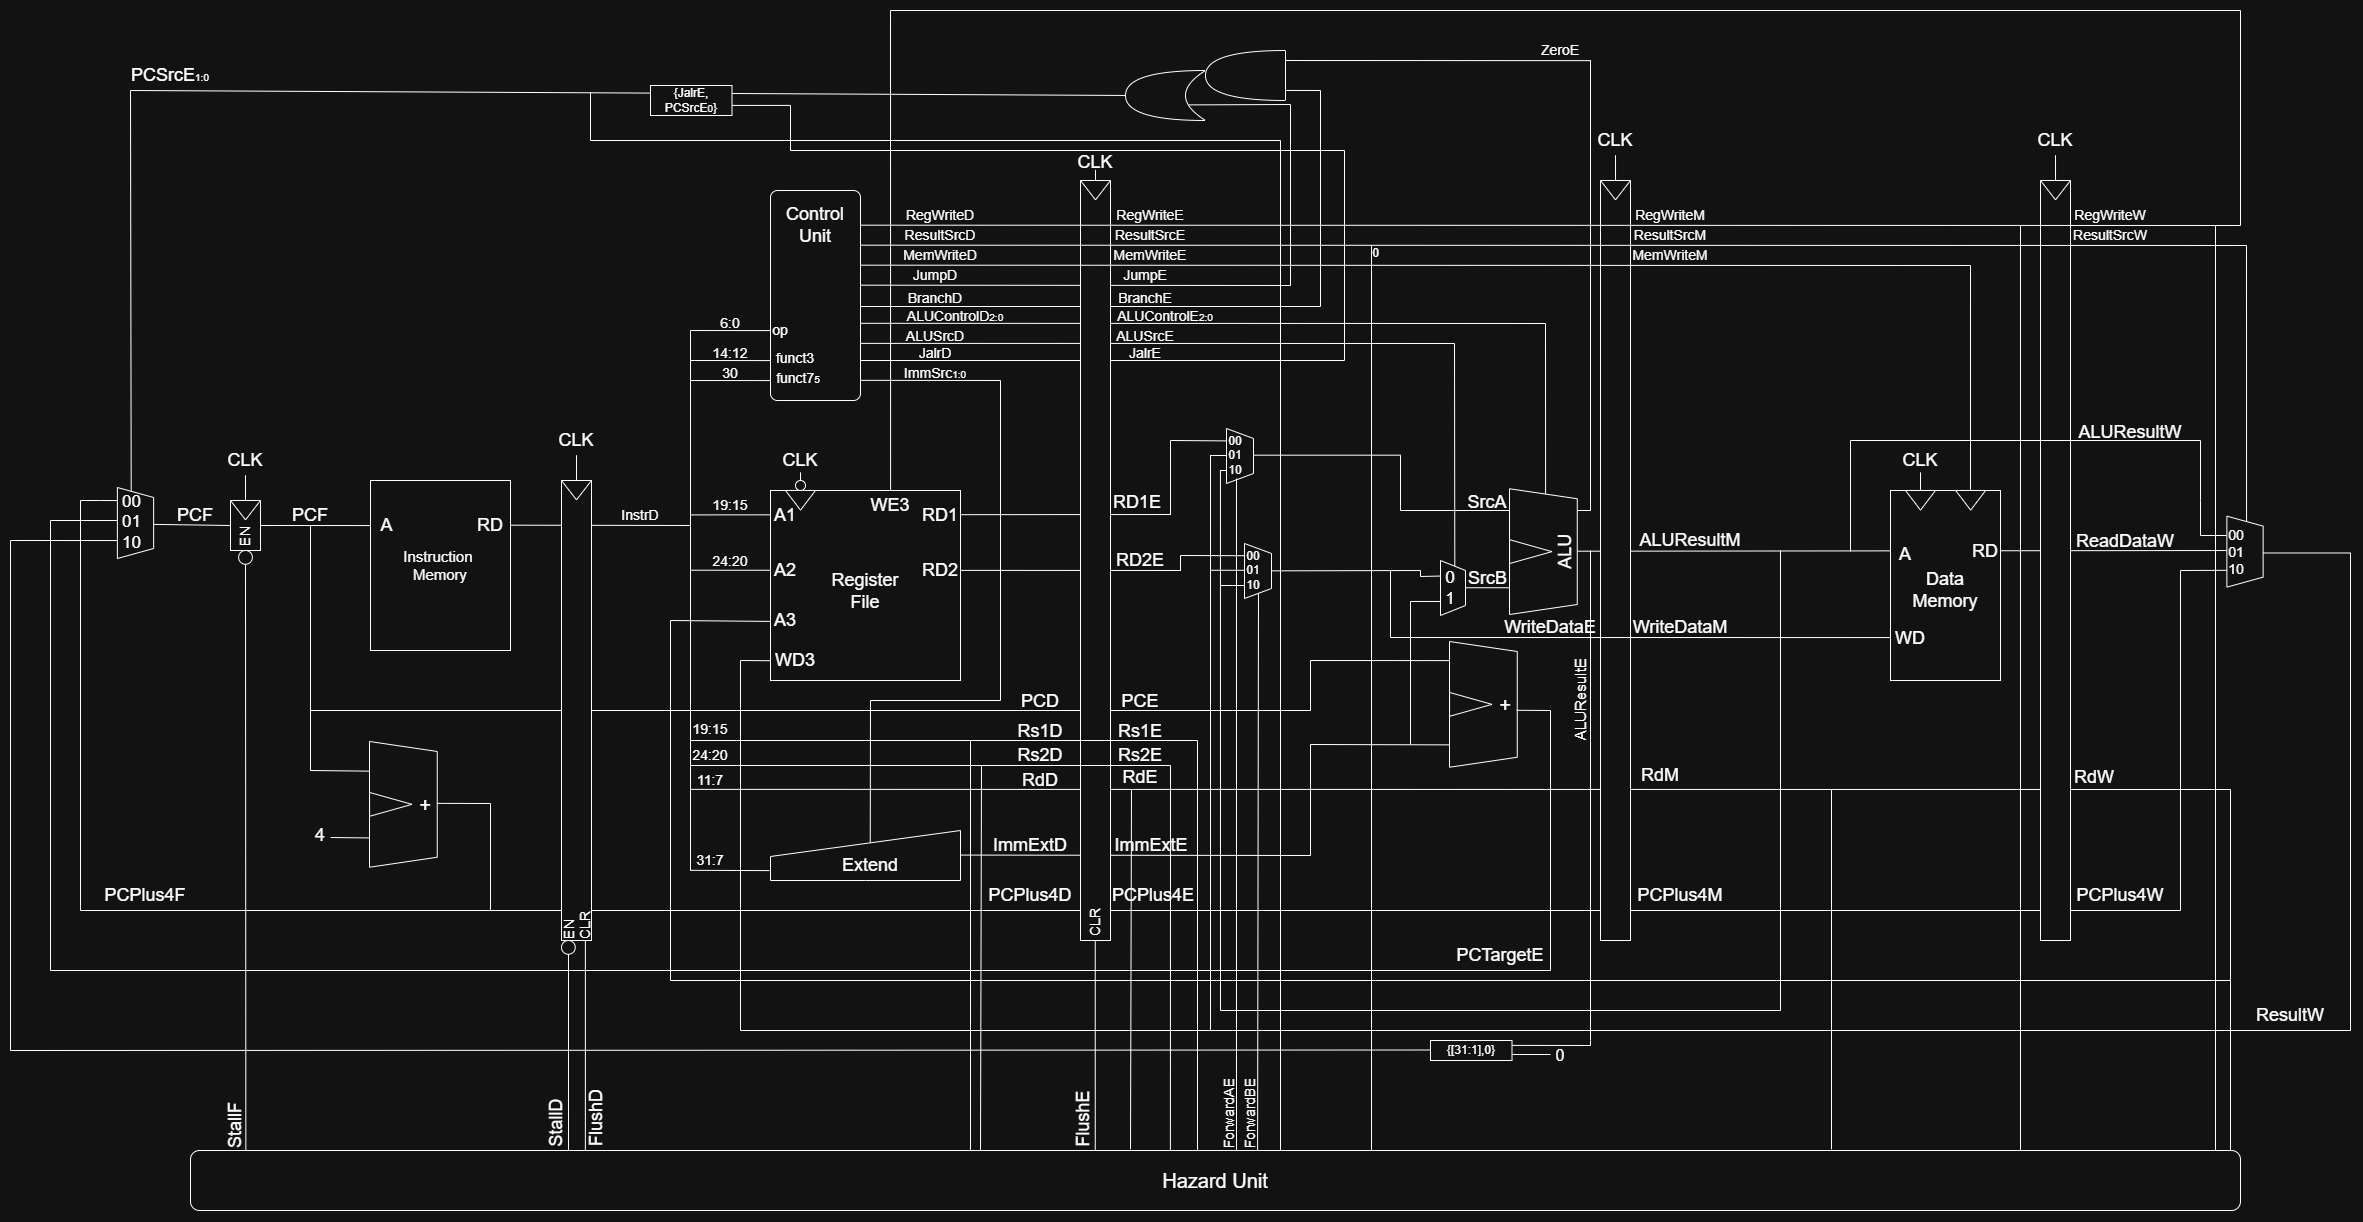
\includegraphics[width=\textwidth]{../img/Pipeline_Single_Issue_Datapath_with_Hazard.jpg}\\[4pt]
\caption{Datapath del pipeline Single-Issue con la Hazard Unit: registros de pipeline, multiplexores de forwarding en EX y señales de stall y flush.}
\label{fig:dp-single}
\end{figure}

El multiplexor del PC tiene tres entradas: \sig{00} para \sig{PC+4}, \sig{01} para el destino de \sig{beq} y \sig{jal} (\sig{PCTargetE}) y \sig{10} para \sig{jalr}, cuyo destino es \sig{ALUResultE} con el bit~0 en cero. El Register File escribe en el flanco de bajada del reloj: así, una instrucción en WB escribe en la primera mitad del ciclo y la que está en ID lee el valor nuevo en la segunda mitad, lo que nos ahorra un caso de forwarding. Cuando el registro IF/ID se anula, se carga un NOP real (\sig{addi x0, x0, 0}) en lugar de ceros, para que el controller nunca decodifique una instrucción inválida.

\begin{vlog}
// PC: 00 = PC+4, 01 = PCTargetE, 10 = jalr (bit 0 en cero)
mux3 #(WIDTH) pcmux(.d0(PCPlus4F), .d1(PCTargetE), .d2({ALUResultE[31:1], 1'b0}),
                    .s(PCSrcE), .y(PCNextF));

// Register File: escribe en el flanco de bajada
always @(negedge clk)
  if (we3) rf[a3] <= wd3;
\end{vlog}

\subsection{Unidad de control}

El controller decodifica en ID con \sig{maindec} y \sig{aludec} y hace viajar cada señal con su instrucción hasta la etapa donde se usa. \sig{ImmSrc} se consume en ID; \sig{ALUSrc}, \sig{ALUControl}, \sig{Branch}, \sig{Jump} y \sig{Jalr} en EX; \sig{MemWrite} en MEM, y \sig{RegWrite} y \sig{ResultSrc} en WB. El salto se resuelve en EX con \texttt{PCSrcE = \{JalrE, (BranchE \& ZeroE) | JumpE\}}. El registro de control ID/EX se limpia con \sig{FlushE}, de modo que una instrucción anulada no escribe registros ni memoria. Respecto al procesador single-cycle original, añadimos la señal \sig{Jalr} a \sig{maindec} (la palabra de control pasó de 11 a 12 bits) para soportar \sig{jalr}:

\begin{vlog}
7'b1100111: controls = 12'b1_00_1_0_10_0_00_0_1; // jalr, en maindec
assign PCSrcE = {JalrE, (BranchE & ZeroE) | JumpE};
\end{vlog}

% =====================================================================
\section{Hazard Unit}
\label{sec:hazard}
% =====================================================================

La Hazard Unit (\sig{hazardunit.v}) se encarga de los tres tipos de riesgo del pipeline.

\textbf{Forwarding.} Si un registro fuente de la instrucción en EX es el destino de una instrucción en MEM o WB que escribe en el Register File, se le pasa el valor directamente. MEM tiene prioridad porque contiene el resultado más reciente:

\begin{vlog}
if      ((Rs1E != 0) && (Rs1E == RdM) && RegWriteM) ForwardAE = 2'b10; // desde MEM
else if ((Rs1E != 0) && (Rs1E == RdW) && RegWriteW) ForwardAE = 2'b01; // desde WB
else                                                ForwardAE = 2'b00;
\end{vlog}

\textbf{Stall (load-use).} Un \sig{lw} recién tiene su dato al final de MEM. Si la instrucción que le sigue lo necesita, se congelan el PC y el registro IF/ID durante un ciclo y se ingresa una burbuja en EX:

\begin{vlog}
assign lwStall = ResultSrcE0 & (RdE != 5'b0) & ((Rs1D == RdE) | (Rs2D == RdE));
assign StallF  = lwStall;
assign StallD  = lwStall;
\end{vlog}

\textbf{Flush.} Para instrucciones del formato B o de salto, el salto se decide en EX, pero para entonces ya entraron dos instrucciones (en IF e ID). Si el salto se toma, ambas se anulan, realizando el Flush con los registros IF/ID e ID/EX:

\begin{vlog}
assign FlushD = |PCSrcE;
assign FlushE = lwStall | (|PCSrcE);
\end{vlog}

\begin{nota}{Error corregido: \sig{jalr} no hacía flush}
La versión original tenía \sig{assign FlushD = PCSrcE;}. \sig{PCSrcE} es de 2~bits y \sig{FlushD} de 1, así que Verilog se quedaba solo con el bit menos significativo. Para \sig{jalr} (\sig{PCSrcE = 10}) eso daba \sig{FlushD = 0}, y las dos instrucciones siguientes se ejecutaban aunque no debían. Lo corregimos con la reducción OR (\sig{|PCSrcE}), que vale 1 ante cualquier salto tomado. El Programa~4 lo comprueba: con la versión anterior, \sig{x14} y \sig{x15} terminaban en 99; con la corregida quedan en~0. También agregamos \sig{RdE != 0} a \sig{lwStall}, porque un \sig{lw} hacia \sig{x0} no debería frenar el pipeline.
\end{nota}

% =====================================================================
\section{Programas de prueba}
% =====================================================================

Cada programa tiene su código Assembly, su archivo \sig{.mem} (verificado contra el ensamblador RISC-V) y un testbench que revisa por sí solo los registros, la memoria y la cantidad de stalls y flushes. La Tabla~\ref{tab:resultados} resume lo obtenido; en las secciones siguientes explicamos cada waveform.

\begin{table}[htbp]
\centering
\caption{Resultados de los programas de prueba sobre el pipeline Single-Issue.}
\label{tab:resultados}
\begin{tabular}{l l l c}
\toprule
\textbf{Programa} & \textbf{Qué prueba} & \textbf{Qué se observa} & \textbf{Testbench} \\
\midrule
1 --- ISA        & Todas las instrucciones, sin dependencias & Sin forwarding, stall ni flush & PASS \\
2 --- Forwarding & Cadena de dependencias RAW     & 4 ciclos con forwarding & PASS \\
3 --- Stalling   & Dependencia load-use           & 1 stall & PASS \\
4 --- Flushing   & \sig{beq}, \sig{jal}, \sig{jalr} & 3 flushes & PASS \\
\bottomrule
\end{tabular}
\end{table}

\subsection{Programa 1: instrucciones sin dependencias}

Este programa recorre todas las instrucciones que soporta el procesador y las ordena para que ninguna necesite a la Hazard Unit: cada instrucción que produce un valor está al menos a tres instrucciones de la que lo usa, distancia a la que el Register File ya tiene el dato gracias a la escritura en flanco de bajada. \sig{jal}, \sig{jalr} y un \sig{beq} tomado no pueden probarse aquí, porque siempre provocan un flush; esos se verifican en el Programa~4. El testbench comprueba los registros \sig{x1} a \sig{x18}, las dos palabras escritas en memoria y que durante todo el programa no haya ningún forwarding, stall ni flush.

\begin{asm}
addi x4, x0, 3      # x4 = 3
addi x1, x0, 12     # x1 = 12
addi x2, x0, 5      # x2 = 5
addi x3, x0, 8      # x3 = 8
                    # 4 NOP
add  x5, x1, x2     # x5 = 17
sub  x6, x3, x4     # x6 = 5
and  x7, x1, x3     # x7 = 8
or   x8, x2, x4     # x8 = 7
xor  x9, x1, x2     # x9 = 9
slt  x10, x4, x2    # x10 = 1   (3 < 5)
addi x11, x0, -5    # x11 = -5
andi x12, x1, 6     # x12 = 4   (12 & 6)
ori  x13, x2, 8     # x13 = 13  (5 | 8)
xori x14, x3, 15    # x14 = 7   (8 ^ 15)
slti x15, x2, 7     # x15 = 1   (5 < 7)
sw   x1, 0(x0)      # Mem[0] = 12
sw   x2, 4(x0)      # Mem[1] = 5
lw   x16, 0(x0)     # x16 = 12
lw   x17, 4(x0)     # x17 = 5
                    # 3 NOP
beq  x16, x17, salto  # 12 != 5: no se toma
addi x18, x0, 1     # x18 = 1
salto:
\end{asm}

\begin{figure}[htbp]
\centering
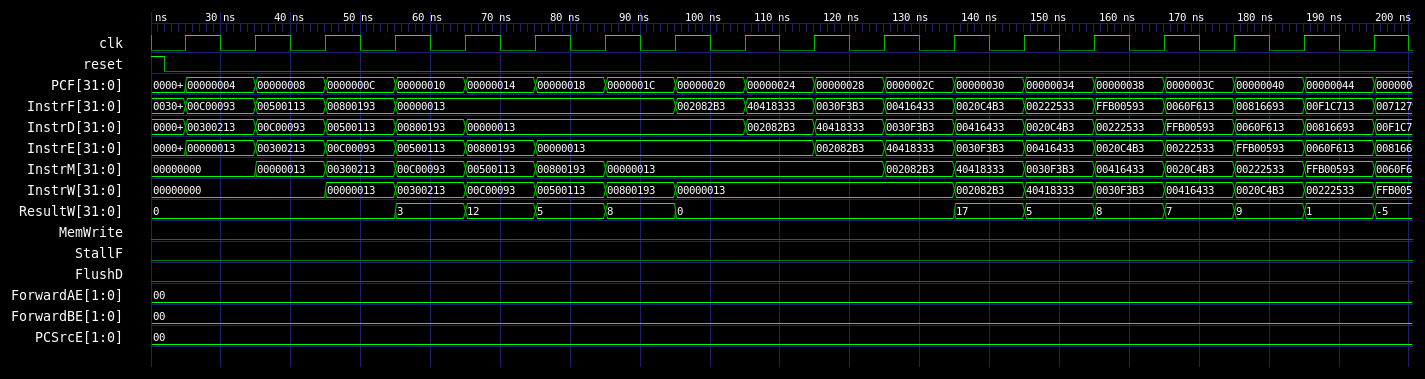
\includegraphics[width=\textwidth]{../img/prog1_isa_a.png}\\[4pt]
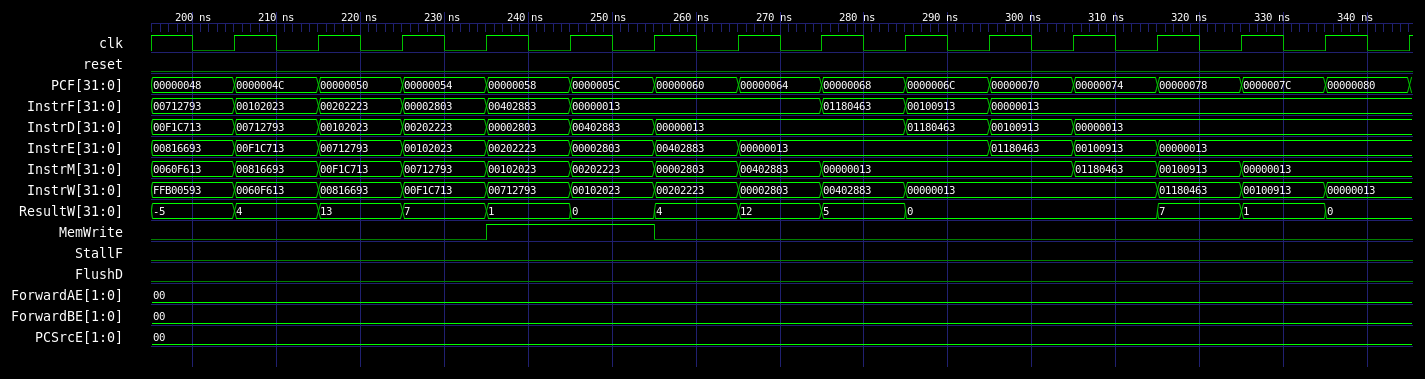
\includegraphics[width=\textwidth]{../img/prog1_isa_b.png}
\caption{Programa 1. Arriba, de 20 a 200~ns; abajo, de 195 a 345~ns.}
\label{fig:p1}
\end{figure}

En la Figura~\ref{fig:p1} se ve el caso ideal del pipeline: cada instrucción baja en diagonal de \sig{InstrF} a \sig{InstrW}, una etapa por ciclo, y el PC avanza de 4 en 4 sin detenerse. \sig{StallF}, \sig{FlushD}, \sig{ForwardAE}, \sig{ForwardBE} y \sig{PCSrcE} se mantienen en 0 durante todo el programa, así que la Hazard Unit nunca interviene. \sig{ResultW} muestra los valores en el orden en que se escriben: 3, 12, 5 y 8 de la inicialización (60--90~ns); 17, 5, 8, 7, 9 y 1 de las instrucciones tipo~R, incluido el \sig{slt} (140--190~ns), y $-5$, 4, 13, 7 y 1 de las instrucciones con inmediato (200--240~ns).

La parte de memoria está en la captura inferior. \sig{MemWrite} sube durante dos ciclos, entre los 235 y 255~ns: son los dos \sig{sw}, que escriben 12 en \sig{Mem[0]} y 5 en \sig{Mem[1]}. A los 270 y 280~ns, \sig{ResultW} muestra 12 y 5, los valores que los \sig{lw} leyeron de esas mismas direcciones. El \sig{beq} llega a EX a los 300~ns; como $12 \neq 5$, \sig{PCSrcE} sigue en \sig{00}, no hay flush, y \sig{addi x18} escribe su 1 a los 330~ns. Los valores 0 y 4 de \sig{ResultW} hacia los 250~ns son las direcciones que calcularon los \sig{sw}, y el 7 de los 320~ns es la resta $12-5$ del \sig{beq}; ninguno se escribe, porque esas instrucciones tienen \sig{RegWrite = 0}.

\subsection{Programa 2: forwarding}

\begin{asm}
addi x1, x0, 5      # x1 = 5
addi x2, x0, 10     # x2 = 10
add  x3, x1, x2     # x3 = 15   (x1 desde WB, x2 desde MEM)
sub  x4, x3, x1     # x4 = 10   (x3 desde MEM)
add  x5, x4, x3     # x5 = 25   (x4 desde MEM, x3 desde WB)
add  x6, x5, x4     # x6 = 35   (x5 desde MEM, x4 desde WB)
\end{asm}

\begin{figure}[htbp]
\centering
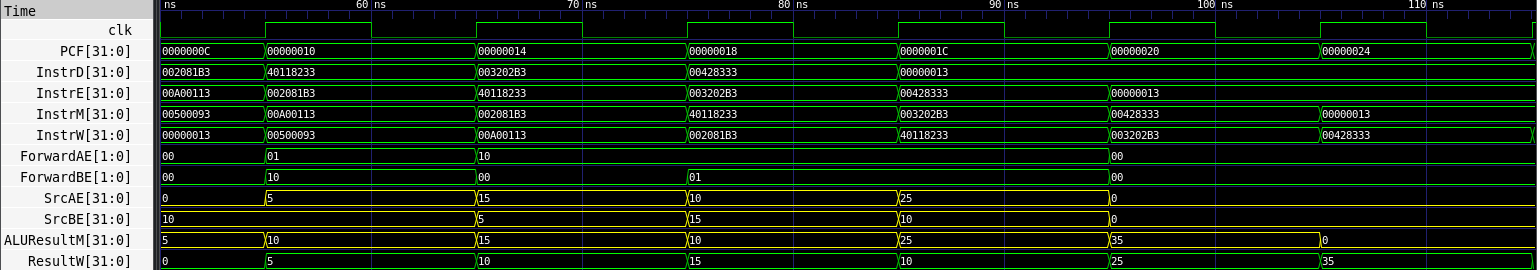
\includegraphics[width=\textwidth]{../img/prog2_forwarding_datos.png}
\caption{Programa 2, de 50 a 115~ns. En amarillo, las señales agregadas para ver los datos, en decimal. Las instrucciones aparecen en ensamblador y \sig{ForwardAE} y \sig{ForwardBE} indican el origen del dato.}
\label{fig:p2}
\end{figure}

Aquí cada instrucción necesita el resultado de la anterior antes de que llegue al Register File. La Tabla~\ref{tab:p2} resume lo que hace el forwarding en cada ciclo de la Figura~\ref{fig:p2}. Ninguna instrucción se detiene: sin forwarding, cada una habría esperado dos ciclos. \sig{ResultW} confirma los valores 15, 10, 25 y 35 entre los 80 y 110~ns.

Para ver el dato que realmente usa la ALU agregamos a la waveform \sig{SrcAE}, \sig{SrcBE} y \sig{ALUResultM}. \sig{SrcAE} y \sig{SrcBE} son las salidas de los multiplexores de forwarding, que eligen el operando según \sig{ForwardAE} y \sig{ForwardBE}:

\begin{vlog}
// 00 = registro, 01 = ResultW (WB), 10 = ALUResultM (MEM)
mux3 #(WIDTH) srcamux(.d0(RD1E), .d1(ResultW), .d2(ALUResultM), .s(ForwardAE), .y(SrcAE));
\end{vlog}

La selección la hace el código de la Sección~\ref{sec:hazard}, y \sig{SrcBE} se obtiene igual con \sig{ForwardBE}. Así, cada operando se comprueba en la Figura~\ref{fig:p2}: a los 60~ns, \sig{ForwardAE = 01} hace que \sig{SrcAE} tome el 5 de \sig{ResultW}, y \sig{ForwardBE = 10} hace que \sig{SrcBE} tome el 10 de \sig{ALUResultM}. La suma da el 15 que aparece en \sig{ALUResultM} a los 70~ns.

\begin{table}[htbp]
\centering
\caption{Forwarding observado en el Programa 2.}
\label{tab:p2}
\small
\begin{tabular}{c l c c c c l}
\toprule
\textbf{Tiempo} & \textbf{En EX} & \sig{ForwardAE} & \sig{ForwardBE} & \sig{SrcAE} & \sig{SrcBE} & \textbf{Origen de los operandos} \\
\midrule
60~ns & \sig{add x3, x1, x2} & 01 & 10 & 5 & 10 & \sig{x1} desde WB, \sig{x2} desde MEM \\
70~ns & \sig{sub x4, x3, x1} & 10 & 00 & 15 & 5 & \sig{x3} desde MEM, \sig{x1} del registro \\
80~ns & \sig{add x5, x4, x3} & 10 & 01 & 10 & 15 & \sig{x4} desde MEM, \sig{x3} desde WB \\
90~ns & \sig{add x6, x5, x4} & 10 & 01 & 25 & 10 & \sig{x5} desde MEM, \sig{x4} desde WB \\
\bottomrule
\end{tabular}
\end{table}

\subsection{Programa 3: stalling por load-use}

\begin{asm}
addi x1, x0, 0      # x1 = 0
addi x2, x0, 10     # x2 = 10
sw   x2, 0(x1)      # Mem[0] = 10
lw   x3, 0(x1)      # x3 = 10
add  x4, x3, x2     # x4 = 20   <- usa x3 justo despues del lw: stall
sub  x5, x4, x2     # x5 = 10
add  x6, x5, x3     # x6 = 20
\end{asm}

\begin{figure}[htbp]
\centering
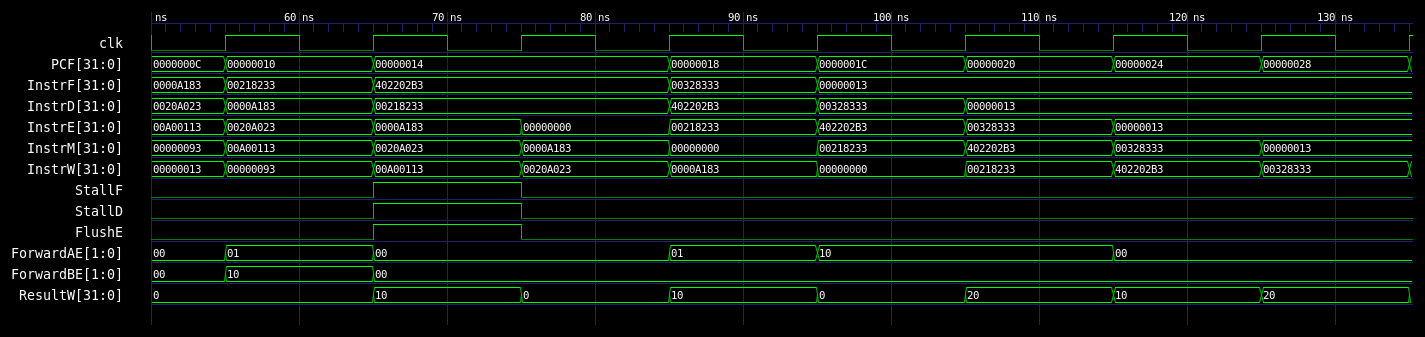
\includegraphics[width=\textwidth]{../img/prog3_stalling.png}
\caption{Programa 3, de 50 a 135~ns.}
\label{fig:p3}
\end{figure}

La Figura~\ref{fig:p3} muestra el único stall del programa. A los 60~ns, el \sig{sw} recibe por forwarding desde MEM el dato que va a guardar (\sig{ForwardBE = 10}). A los 70~ns el \sig{lw x3} está en EX y el \sig{add x4, x3, x2} en ID; como \sig{x3} recién estará listo al final de MEM, la Hazard Unit levanta a la vez \sig{StallF}, \sig{StallD} y \sig{FlushE}. El efecto se ve claro a los 80~ns: \sig{PCF} sigue en \sig{0x14} e \sig{InstrD} sigue siendo el \sig{add}, porque ambos quedaron congelados, mientras \sig{InstrE} vale 0, que es la burbuja insertada.

Un ciclo después, a los 90~ns, el \sig{add} entra a EX y toma \sig{x3 = 10} desde WB (\sig{ForwardAE = 01}), porque el \sig{lw} ya leyó la memoria. Las dos instrucciones siguientes obtienen su operando desde MEM (\sig{ForwardAE = 10}) sin más esperas. Un ciclo de stall es el costo mínimo de una dependencia load-use en este pipeline.

\subsection{Programa 4: flushing}

\begin{asm}
      addi x1, x0, 5
      addi x2, x0, 5
      addi x3, x0, 7
      beq  x1, x3, t1     # NO se toma (5 != 7)
      addi x4, x0, 1      # x4 = 1
      beq  x1, x2, t1     # se toma -> flush
      addi x5, x0, 99     # anulada
      addi x6, x0, 99     # anulada
t1:   addi x7, x0, 2
      jal  x8, t2         # x8 = 40 -> flush
      addi x9, x0, 99     # anulada
      addi x10, x0, 99    # anulada
t2:   addi x11, x0, 3
      addi x12, x0, 68
      jalr x13, 0(x12)    # x13 = 60 -> flush
      addi x14, x0, 99    # anulada
      addi x15, x0, 99    # anulada
t3:   addi x16, x0, 4
      sw   x16, 0(x0)
fin:  beq  x0, x0, fin
\end{asm}

\begin{figure}[htbp]
\centering
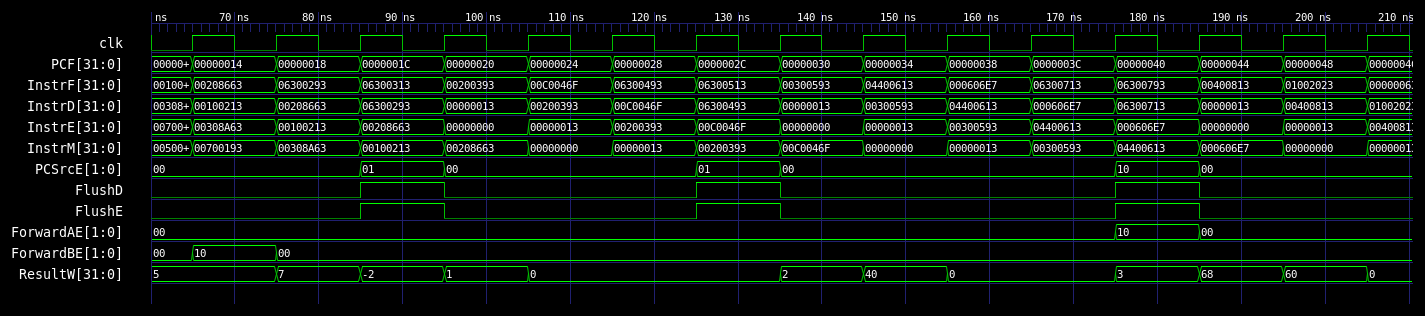
\includegraphics[width=\textwidth]{../img/prog4_flushing.png}
\caption{Programa 4, de 60 a 210~ns.}
\label{fig:p4}
\end{figure}

El programa recorre los tres tipos de salto. En la Figura~\ref{fig:p4}, a los 70~ns el primer \sig{beq} está en EX y recibe \sig{x3} por forwarding (\sig{ForwardBE = 10}); como $5 \neq 7$, \sig{PCSrcE} queda en \sig{00} y no pasa nada: \sig{addi x4} sigue su camino.

A los 90~ns el segundo \sig{beq} sí se toma. \sig{PCSrcE} pasa a \sig{01} y se activan \sig{FlushD} y \sig{FlushE}, que anulan las dos \sig{addi ..., 99} que estaban en ID e IF. En el ciclo siguiente se ve el resultado: \sig{InstrD} es un NOP, \sig{InstrE} vale 0 y \sig{PCF} ya apunta a \sig{0x20} (\sig{t1}). El \sig{jal} de los 130~ns se comporta igual, y a los 150~ns \sig{ResultW} muestra el 40 que se guarda en \sig{x8} como dirección de retorno.

El caso más interesante es el \sig{jalr} de los 180~ns. Recibe \sig{x12 = 68} por forwarding desde MEM (\sig{ForwardAE = 10}), pone \sig{PCSrcE = 10} y esta vez sí provoca el flush, que es justamente lo que fallaba antes de la corrección. A los 190~ns el PC ya está en \sig{0x44} (\sig{t3}) y a los 200~ns \sig{ResultW} muestra el 60 de \sig{x13}.

El $-2$ que aparece en \sig{ResultW} hacia los 90~ns no es un error: es la resta $5-7$ que hizo el \sig{beq} no tomado al llegar a WB, y no se escribe en ningún registro porque \sig{beq} tiene \sig{RegWrite = 0}. Cada salto tomado cuesta dos ciclos, uno por cada instrucción anulada.

% =====================================================================
\section{Primeros pasos hacia Dual-Issue}
% =====================================================================

En esta entrega construimos la parte frontal del procesador Dual-Issue: leer y decodificar dos instrucciones por ciclo. La ejecución en paralelo (Issue Unit y segunda ALU) queda para E2. La Figura~\ref{fig:dp-dual} resume los cambios.

\textbf{Dual Fetch.} A la memoria de instrucciones le agregamos un segundo puerto de lectura: \sig{rd} entrega la instrucción en \sig{PC} y \sig{rd1} la de \sig{PC+4}. Como en cada lectura llega un par, el PC avanza de 8 en 8. El PC se actualiza cuando el par que está en Decode ya terminó de emitirse o cuando hay un salto tomado.

\begin{vlog}
assign rd  = RAM[a[31:2]];     // imem: instruccion en PC
assign rd1 = RAM[a[31:2] + 1]; // imem: instruccion en PC+4
.en(~StallF & (SelD | FlushD)) // habilitacion del registro del PC
\end{vlog}

\textbf{Dual Decode.} El registro IF/ID ahora es doble y guarda \sig{InstrD0} (slot~0, la instrucción más antigua), \sig{InstrD1} (slot~1) y el PC base del par. El controller tiene dos decodificadores (dos \sig{maindec} y dos \sig{aludec}) y el datapath dos unidades \sig{extend}, así que ambas instrucciones se decodifican en el mismo ciclo. El Register File pasó a tener cuatro puertos de lectura y dos de escritura: lee \sig{rs1} y \sig{rs2} de las dos instrucciones a la vez. El segundo puerto de escritura ya existe y, si las dos vías escriben el mismo registro, gana la vía~1 por ser la instrucción más joven; lo conectaremos en E2.

\begin{vlog}
always @(negedge clk) begin
  if (we3)  rf[a3] <= wd3;
  if (web3) rf[b3] <= wdb3;   // va despues: tiene prioridad
end
\end{vlog}

\textbf{Módulos de la vía 1.} También instanciamos el registro ID/EX de la vía 1 (\sig{regE1}, con los operandos, el inmediato y el control del slot~1) y su ALU (\sig{alu1}), con su propio multiplexor de \sig{ALUSrc}. En esta entrega la señal \sig{Issue1D} está fija en 0, de modo que ese registro se limpia en cada ciclo y la vía 1 solo procesa burbujas. En E2 la Issue Unit pondrá \sig{Issue1D} en 1 cuando las dos instrucciones del par puedan salir juntas.

\textbf{Emisión.} Como E1 todavía no pide ejecutar dos instrucciones a la vez, emitimos una por ciclo y en orden. La señal \sig{SelD} elige el slot: con \sig{SelD = 0} sale la instrucción más antigua del par y con \sig{SelD = 1} la más joven; después entra el siguiente par. A EX pasan el control y los operandos del slot elegido. Esta idea de guardar la instrucción más joven para el ciclo siguiente es la base del reagrupamiento que hará la Issue Unit en E2. Ante un salto tomado se limpia el par en Decode, y si el salto estaba en el slot~0, la instrucción del slot~1 se anula con \sig{FlushE}.

\begin{vlog}
assign InstrD = SelD ? InstrD1 : InstrD0;   // slot que se emite
assign PCD    = PCPairD + {SelD, 2'b00};
\end{vlog}

\begin{figure}[htbp]
\centering
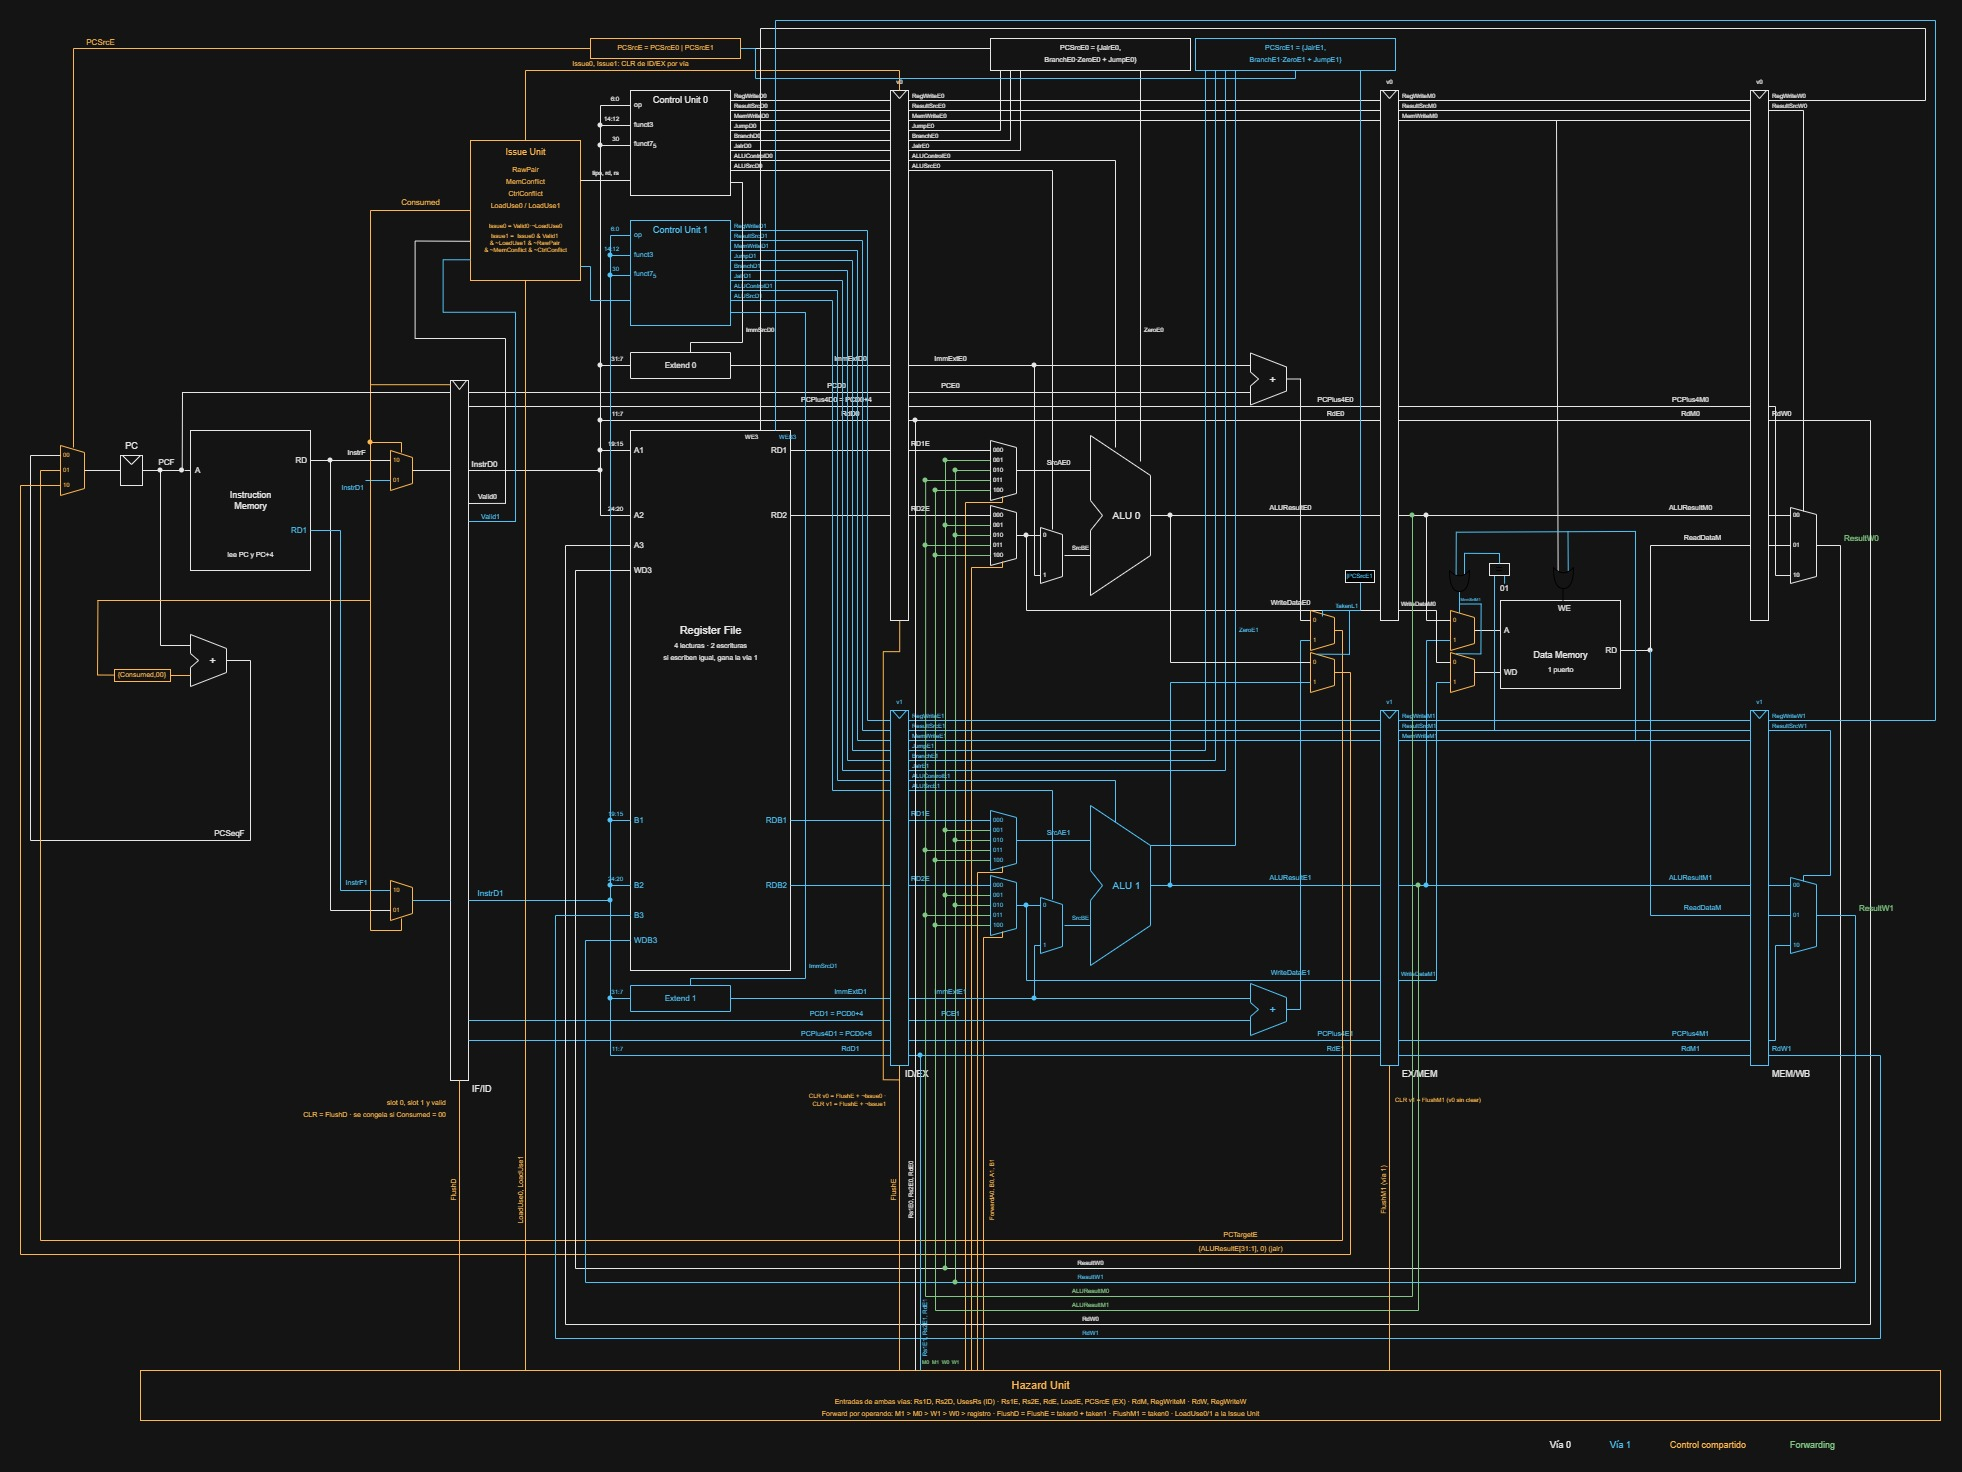
\includegraphics[width=\textwidth]{../img/datapath_dual_issue_v2.jpg}
\caption{Datapath Dual-Issue preliminar. Arriba la vía~0 y abajo la vía~1; cada registro de pipeline está partido en una sección por vía. En blanco, lo que se mantiene del Single-Issue (Figura~\ref{fig:dp-single}); en celeste, lo agregado en E1 para leer y decodificar el par; en gris punteado, la vía~1 después de Decode, que ya tiene su registro ID/EX y su ALU pero en E1 solo recibe burbujas.}
\label{fig:dp-dual}
\end{figure}

\subsection{Programa 5: evidencia de Dual Fetch y Dual Decode}

\begin{asm}
      addi x1, x0, 1      # par 0x00
      addi x2, x0, 2
      addi x3, x0, 3      # par 0x08
      addi x4, x0, 4
      add  x5, x1, x2     # par 0x10
      add  x6, x3, x4
      sw   x5, 0(x0)      # par 0x18
      sw   x6, 4(x0)
      beq  x0, x0, t1     # par 0x20: salto tomado en el slot 0
      addi x7, x0, 99     #           el slot 1 se anula
t1:   addi x8, x0, 8
fin:  beq  x0, x0, fin
\end{asm}

El testbench de este programa revisa cinco cosas: que el par leído sea siempre (PC, PC+4); que sin saltos el PC avance de 8 en 8; que después de cada salto el PC tome el destino correcto; que las 11 instrucciones válidas lleguen a EX en orden, sin perderse ni repetirse, y que registros y memoria terminen con los valores esperados. Los cuatro programas anteriores también pasan sin cambios sobre esta versión, así que el Dual Fetch y el Dual Decode no alteraron el comportamiento del procesador.

\begin{figure}[htbp]
\centering
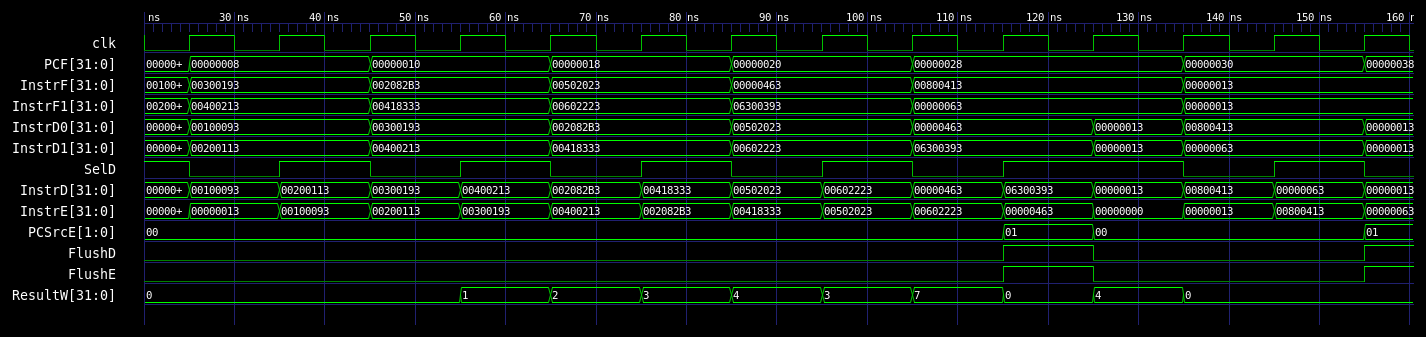
\includegraphics[width=\textwidth]{../img/prog5_dualfetch.png}
\caption{Programa 5, de 20 a 160~ns.}
\label{fig:p5}
\end{figure}

En la Figura~\ref{fig:p5} se ve el ritmo del Dual Fetch. A los 30~ns, Decode tiene el par \sig{0x00} (\sig{InstrD0 = addi x1}, \sig{InstrD1 = addi x2}) y, al mismo tiempo, Fetch ya está leyendo el par \sig{0x08} (\sig{InstrF = addi x3}, \sig{InstrF1 = addi x4}). Con \sig{SelD = 0} sale \sig{addi x1}; a los 40~ns, con \sig{SelD = 1}, sale \sig{addi x2}, mientras el PC y el par de Fetch esperan. A los 50~ns entra el par \sig{0x08} a Decode y \sig{PCF} salta de \sig{0x08} a \sig{0x10}. El patrón se repite cada dos ciclos: un par leído y decodificado, dos instrucciones emitidas.

El salto aparece a los 110~ns, cuando entra el par \sig{0x20} con el \sig{beq} en el slot~0 y \sig{addi x7, 99} en el slot~1. El \sig{beq} se emite primero y a los 120~ns se resuelve tomado en EX (\sig{PCSrcE = 01}) justo cuando se está emitiendo \sig{addi x7}. \sig{FlushE} la anula (a los 130~ns \sig{InstrE} vale 0) y \sig{FlushD} limpia el par. A los 140~ns entra el par destino (\sig{addi x8} y \sig{beq fin}) y todo sigue en orden.

\begin{nota}{Un error que encontramos con este programa}
Al revisar la simulación vimos que, si un salto se tomaba mientras se emitía el slot~0, el PC no saltaba: solo se actualizaba cuando \sig{SelD = 1}, y el destino se perdía. Lo corregimos permitiendo que el PC se actualice también cuando hay un salto tomado (\sig{en = ~StallF & (SelD | FlushD)}), y agregamos al testbench la verificación del destino después de cada salto, que con la versión anterior falla.
\end{nota}

% =====================================================================
\section{Conclusiones}
% =====================================================================

El pipeline de cinco etapas ejecuta correctamente el subconjunto RV32I que soporta y resuelve los tres riesgos del pipeline: forwarding desde MEM y WB, un ciclo de stall ante load-use y la anulación de dos instrucciones en cada salto tomado. Las pruebas automáticas fueron clave: gracias a ellas encontramos dos errores, el flush que faltaba en \sig{jalr} y la pérdida del destino del salto en el Dual Fetch, que con una revisión visual de las waveforms habrían sido fáciles de pasar por alto.

La base del Dual-Issue ya está: Fetch y Decode trabajan con pares de instrucciones y el Register File tiene los cuatro puertos de lectura y dos de escritura que se van a necesitar. La vía 1 ya tiene su registro ID/EX y su ALU. Para E2 queda lo más interesante: completar esa vía hasta WB, la Issue Unit que decida si dos instrucciones pueden salir juntas (dependencias RAW dentro del par y recursos compartidos de memoria y branch) y el forwarding entre vías.

\appendix
\section{Cómo reproducir las pruebas en Vivado}

El código entregado tiene dos carpetas: \sig{Single_Issue}, con la arquitectura A, y \sig{Dual_Issue}, con el avance hacia B. Dentro de cada una hay una carpeta por programa con su código Assembly, su archivo \sig{.mem} y su testbench (Tabla~\ref{tab:repro}). Los programas 1 a 4 también pasan sin cambios en \sig{Dual_Issue}.

\begin{table}[htbp]
\centering
\small
\caption{Archivos de cada prueba.}
\label{tab:repro}
\begin{tabular}{l l l l l}
\toprule
\textbf{Programa} & \textbf{Código} & \textbf{Carpeta} & \textbf{Testbench} & \textbf{Programa cargado} \\
\midrule
1 (ISA)        & \sig{Single_Issue} & \sig{Programa1_ISA}        & \sig{tb_isa.v}        & \sig{isa.mem} \\
2 (Forwarding) & \sig{Single_Issue} & \sig{Programa2_Forwarding} & \sig{tb_forwarding.v} & \sig{forwarding.mem} \\
3 (Stalling)   & \sig{Single_Issue} & \sig{Programa3_Stalling}   & \sig{tb_stalling.v}   & \sig{stalling.mem} \\
4 (Flushing)   & \sig{Single_Issue} & \sig{Programa4_Flushing}   & \sig{tb_flushing.v}   & \sig{flushing.mem} \\
5 (Dual Fetch) & \sig{Dual_Issue}   & \sig{Programa5_DualFetch}  & \sig{tb_dualfetch.v}  & \sig{dualfetch.mem} \\
\bottomrule
\end{tabular}
\end{table}

Los programas 1 a 4 comparten un mismo proyecto de Vivado. El Programa~5 necesita otro, porque usa el código de \sig{Dual_Issue}.

\paragraph{Crear el proyecto.}
\begin{enumerate}
  \item Crear un proyecto RTL nuevo en Vivado.
  \item En \textit{Add Sources} $\to$ \textit{design sources}, agregar todos los \sig{.v} sueltos de \sig{Single_Issue} (los que no están dentro de una carpeta \sig{Programa}). Para el Programa~5 se usan los de \sig{Dual_Issue}.
\end{enumerate}

\paragraph{Simular un programa.}
\begin{enumerate}
  \item En \textit{Add Sources} $\to$ \textit{simulation sources}, agregar el testbench y el \sig{.mem} del programa según la Tabla~\ref{tab:repro}. Para el Programa~1 son \sig{Programa1_ISA/tb_isa.v} y \sig{Programa1_ISA/isa.mem}.
  \item Comprobar que el testbench quedó como top: en \textit{Simulation Sources} aparece en negrita. Si hay más de un testbench en el proyecto, Vivado puede haber elegido otro; en ese caso, clic derecho sobre el correcto y \textit{Set as Top}.
  \item \textit{Run Simulation} $\to$ \textit{Run Behavioral Simulation}. La simulación termina sola y la consola Tcl muestra \sig{PASS} o \sig{FAIL}.
  \item Cerrar la simulación (\textit{Close Simulation}) y repetir los pasos con el siguiente programa de la tabla.
\end{enumerate}

La waveform ya muestra \sig{PCF}, \sig{InstrF} a \sig{InstrW} y las señales de la Hazard Unit, porque el testbench las declara en su nivel superior, así que no hay que agregarlas a mano.

\entrega{Entrega 2}

\renewcommand{\thesection}{\arabic{section}}
\setcounter{section}{0}
\renewcommand{\theHsection}{e2.\arabic{section}}

% =====================================================================
\section{Arquitectura Dual-Issue}
% =====================================================================

En esta entrega el procesador ya ejecuta dos instrucciones por ciclo cuando es posible. Conserva las cinco etapas y emite en orden: la instrucción más antigua (slot~0) va por la vía~0 y la más joven (slot~1) por la vía~1. Los sufijos 0 y 1 de las señales indican la vía. La Figura~\ref{fig:dp-e2} muestra el datapath completo.

\begin{figure}[htbp]
\centering
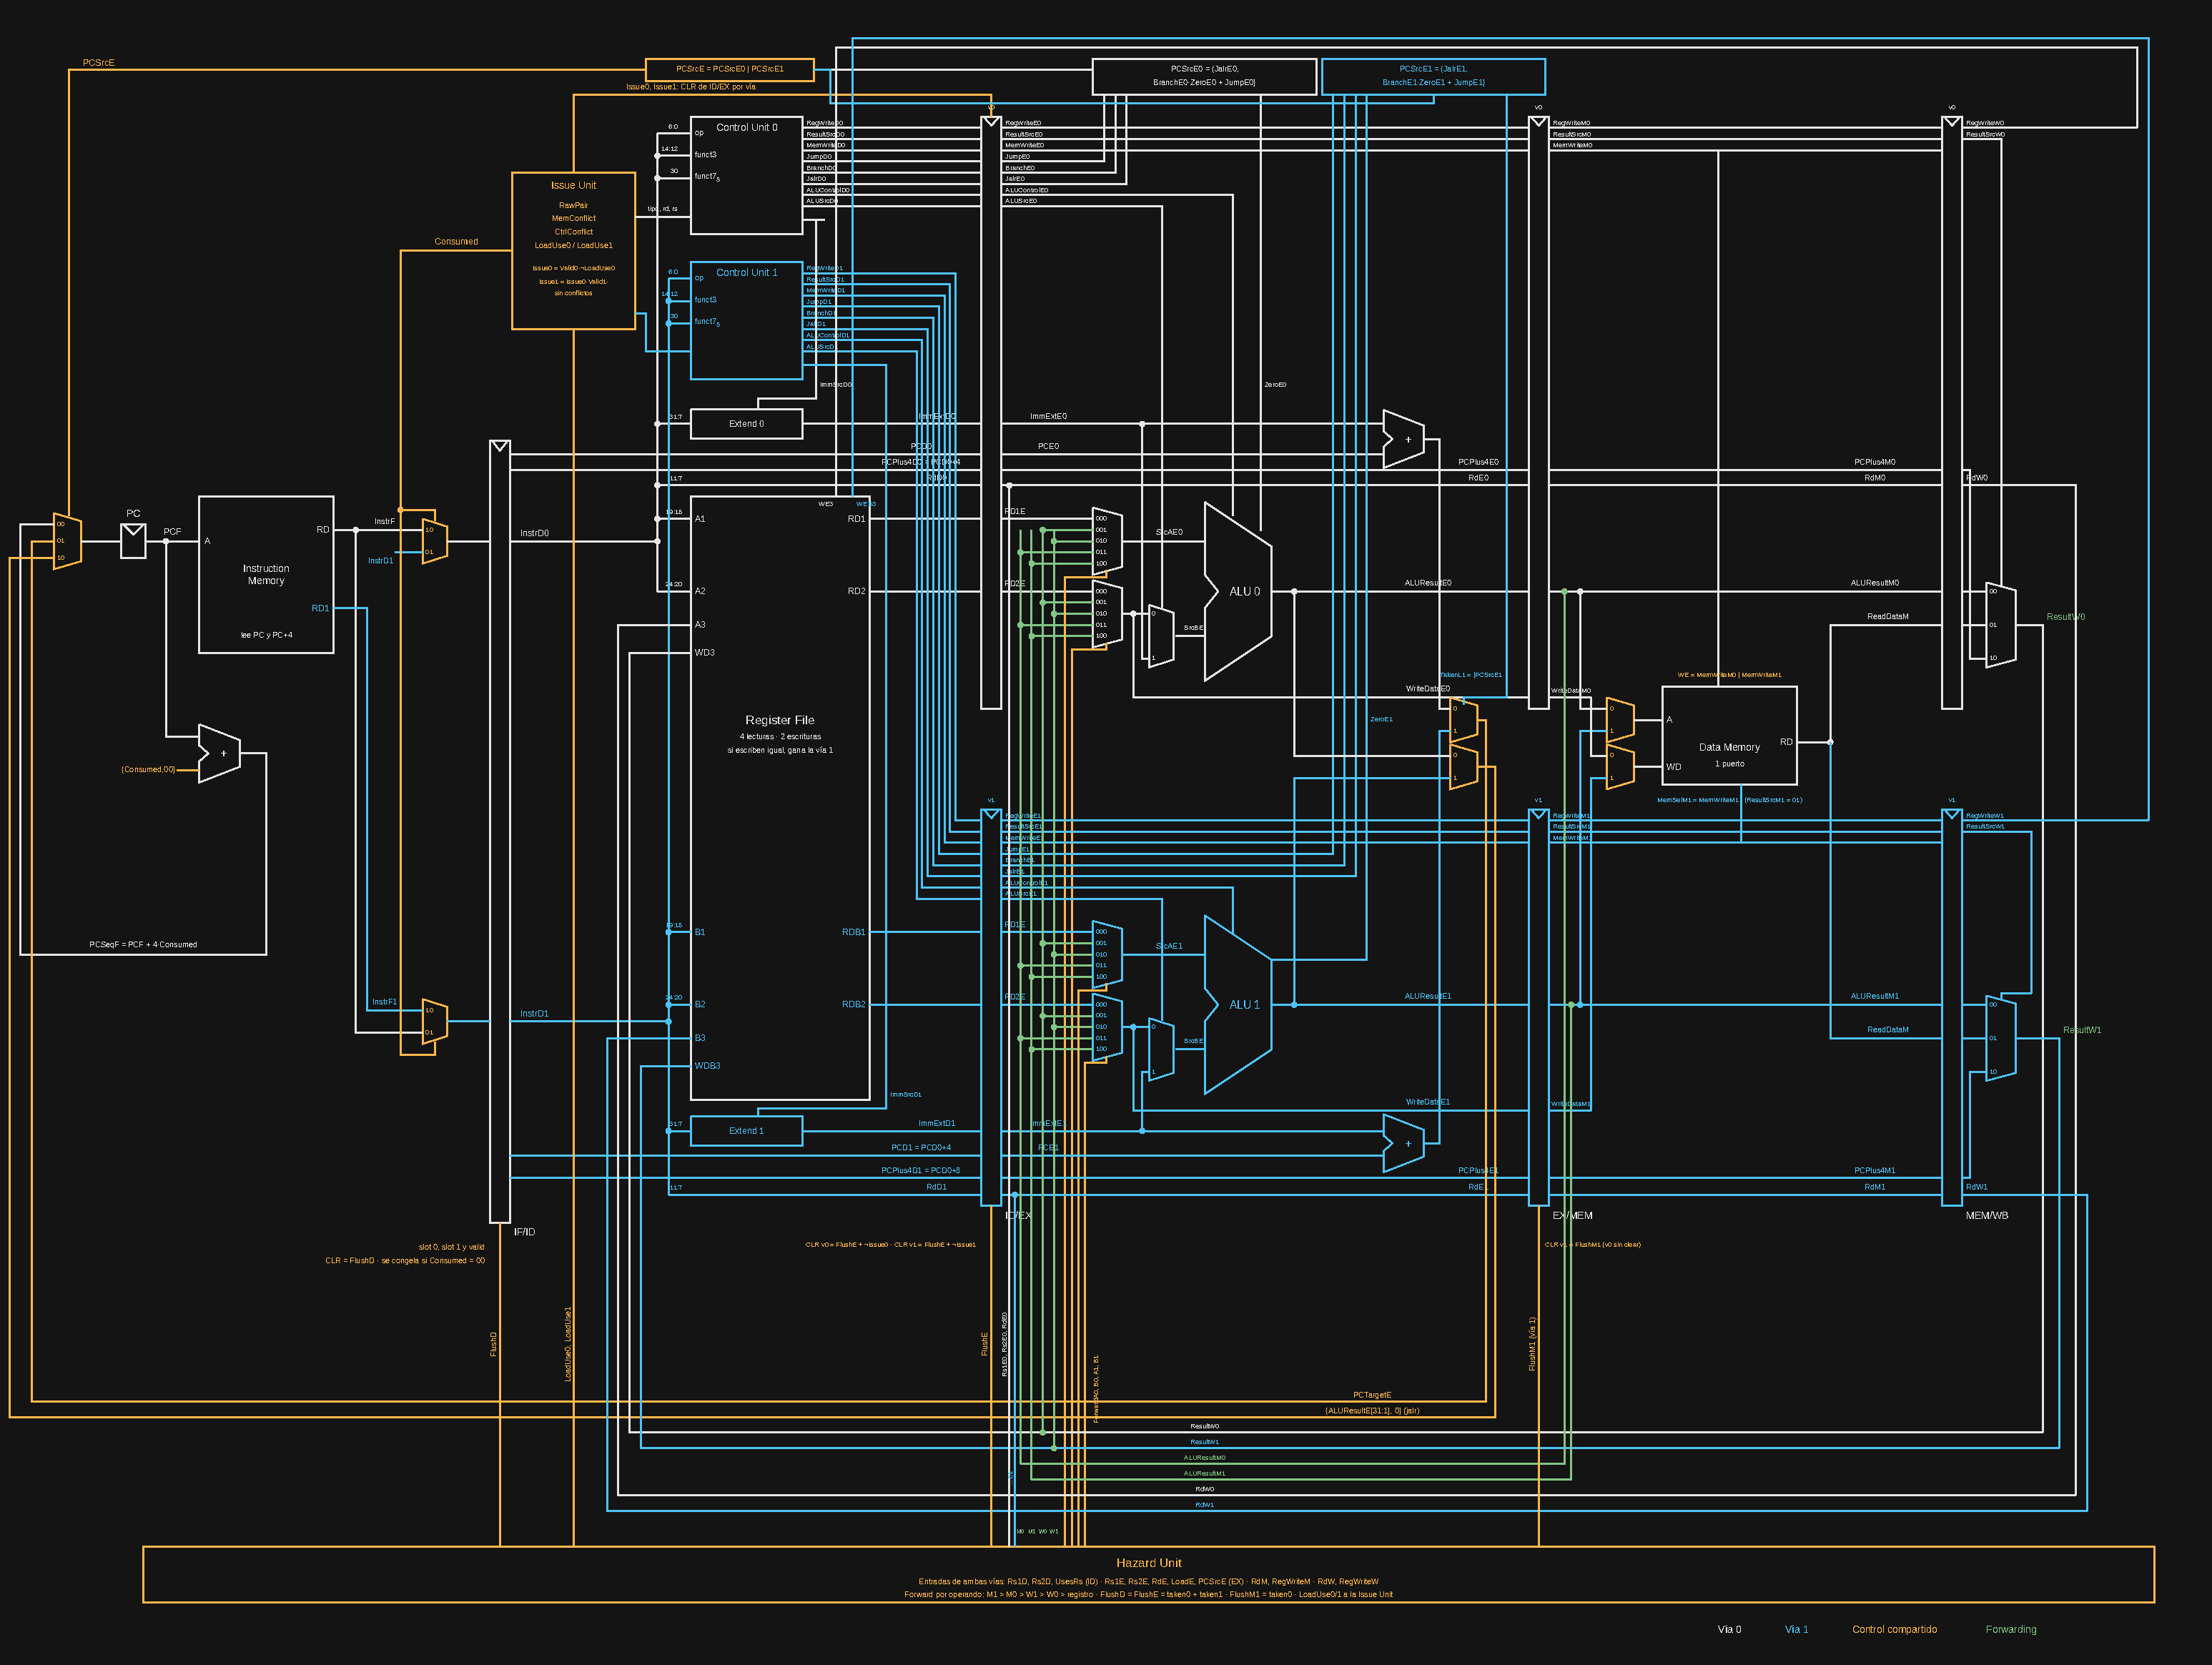
\includegraphics[width=\textwidth]{../img/datapath_dual_issue_e2.pdf}
\caption{Datapath Dual-Issue completo. Arriba la vía~0 (blanco) y abajo la vía~1 (celeste), cada una con sus propios registros ID/EX, EX/MEM y MEM/WB; el registro IF/ID guarda el par de instrucciones. En naranja, la Issue Unit, la Hazard Unit y lo que comparten las dos vías: el resolutor de saltos y la memoria de datos. En verde, los caminos de forwarding.}
\label{fig:dp-e2}
\end{figure}


\textbf{Fetch.} Se leen siempre dos instrucciones consecutivas, y el PC avanza 4 bytes por cada instrucción consumida:

\begin{vlog}
adder pcadd(.a(PCF), .b({28'b0, Consumed, 2'b00}), .y(PCSeqF));
\end{vlog}

\textbf{IF/ID como ventana deslizante.} El registro guarda dos instrucciones y un bit de validez por slot. Reemplaza al \sig{SelD} de E1: si solo sale el slot~0, el slot~1 pasa a ser el slot~0 y se reagrupa con la instrucción siguiente:

\begin{vlog}
end else if (Consumed == 2'b10) begin       // salieron los dos slots
  InstrD0_r <= InstrF;  InstrD1_r <= InstrF1;  PCD0_r <= PCF;
end else if (Consumed == 2'b01) begin       // solo salio el slot 0
  InstrD0_r <= InstrD1_r;  InstrD1_r <= InstrF;  PCD0_r <= PCD0_r + 4;
end                                         // Consumed = 0: la ventana se congela
\end{vlog}

\textbf{Recursos por vía.} Hay dos ALU, dos registros ID/EX, EX/MEM y MEM/WB, y un Register File de cuatro lecturas y dos escrituras (Sección~5 de la Entrega~1). Si ambas vías escriben el mismo registro, gana la vía~1.

\textbf{Recursos compartidos.} La memoria de datos tiene un solo puerto, y un multiplexor se lo entrega a la vía que tenga el load o store. También hay un solo resolutor de saltos, que toma el destino de la vía que tiene el salto:

\begin{vlog}
assign MemSelM1 = MemWriteM1 | (ResultSrcM1 == 2'b01);  // puerto de memoria
wire   TakenL1  = |PCSrcE1;                             // destino del salto
\end{vlog}

\textbf{Controller.} Decodifica las dos instrucciones y lleva un registro de control por vía. Además informa a la Issue Unit qué registros usa cada instrucción, para no crear dependencias falsas: \sig{addi}, por ejemplo, no usa \sig{rs2}. La principal novedad respecto a E1 es que cada vía calcula su propio \sig{PCSrc}.

\begin{table}[htbp]
\centering
\caption{Módulos nuevos y modificados respecto a E1.}
\label{tab:modulos}
\begin{tabularx}{\textwidth}{l l X}
\toprule
\textbf{Módulo} & \textbf{Estado} & \textbf{Cambio} \\
\midrule
\sig{issueunit.v} & Nuevo & Decide la emisión y cuántos slots avanza la ventana. \\
\sig{fwdsel.v} & Nuevo & Selector de forwarding de un operando. \\
\sig{mux5.v} & Nuevo & Multiplexor de forwarding de cinco entradas. \\
\sig{datapath.v} & Modificado & Ventana IF/ID, dos vías completas y puerto de memoria compartido. \\
\sig{controller.v} & Modificado & Control por vía y datos para la Issue Unit. \\
\sig{hazardunit.v} & Modificado & Cuatro forwardings, load-use por slot y flush por vía. \\
\sig{riscvpipeline.v} & Modificado & Conecta la Issue Unit y las señales de las dos vías. \\
\sig{imem.v}, \sig{dmem.v} & Modificado & Memorias ampliadas a 256 palabras. \\
\bottomrule
\end{tabularx}
\end{table}


% =====================================================================
\section{Issue Unit}
% =====================================================================

La Issue Unit (\sig{issueunit.v}) decide en ID cuántas instrucciones del par salen en el ciclo. El slot~1 nunca sale sin el slot~0, así se conserva el orden del programa:

\begin{vlog}
assign RawPair = RegWriteD0 & (RdD0 != 5'b0) &
                 ((UsesRs1D1 & (Rs1D1 == RdD0)) | (UsesRs2D1 & (Rs2D1 == RdD0)));
assign MemConflict  = IsMemD0  & IsMemD1;
assign CtrlConflict = IsCtrlD0 & IsCtrlD1;

assign Issue0 = Valid0 & ~LoadUse0;
assign Issue1 = Issue0 & Valid1 & ~LoadUse1 & ~RawPair & ~MemConflict & ~CtrlConflict;
\end{vlog}

\begin{table}[htbp]
\centering
\caption{Condiciones que impiden emitir el par.}
\label{tab:issue}
\begin{tabularx}{\textwidth}{l X l}
\toprule
\textbf{Señal} & \textbf{Condición} & \textbf{Efecto} \\
\midrule
\sig{RawPair} & El slot~1 lee el registro que escribe el slot~0. & Sale solo el slot~0 \\
\sig{MemConflict} & Los dos son load o store: hay un solo puerto. & Sale solo el slot~0 \\
\sig{CtrlConflict} & Los dos son saltos: hay un solo resolutor. & Sale solo el slot~0 \\
\sig{LoadUse1} & El slot~1 usa el dato de un \sig{lw} que está en EX. & Sale solo el slot~0 \\
\sig{LoadUse0} & El slot~0 usa el dato de un \sig{lw} que está en EX. & No sale ninguno \\
\bottomrule
\end{tabularx}
\end{table}

\textbf{Asignación de recursos.} La instrucción se queda en la vía de su slot, sin importar su tipo. Como ambas vías tienen ALU y acceso al puerto de memoria y al resolutor, una ALU puede salir junto con un load o store, o con un salto, en cualquier orden.

\textbf{Reagrupamiento.} La señal \sig{Consumed} indica cuántas posiciones avanza la ventana. Un slot inválido cuenta como consumido, y por eso la ventana se recarga sola después de un reset o un flush:

\begin{vlog}
wire consumed0 = Issue0 | ~Valid0;
wire consumed1 = Issue1 | ~Valid1;
assign Consumed = consumed0 ? (consumed1 ? 2'b10 : 2'b01) : 2'b00;
\end{vlog}

% =====================================================================
\section{Forwarding, stalls y control de saltos}
% =====================================================================

\textbf{Forwarding.} Cada uno de los cuatro operandos de EX tiene un multiplexor de cinco entradas y su propio selector. Cuando varios productores escriben el mismo registro, gana el más reciente: primero MEM y luego WB, y dentro de cada etapa, la vía~1:

\begin{vlog}
if      ((Rs != 5'b0) && RegWriteM1 && (Rs == RdM1)) Forward = 3'b100; // MEM via 1
else if ((Rs != 5'b0) && RegWriteM0 && (Rs == RdM0)) Forward = 3'b011; // MEM via 0
else if ((Rs != 5'b0) && RegWriteW1 && (Rs == RdW1)) Forward = 3'b010; // WB via 1
else if ((Rs != 5'b0) && RegWriteW0 && (Rs == RdW0)) Forward = 3'b001; // WB via 0
else                                                 Forward = 3'b000; // registro
\end{vlog}

\textbf{Stall por load-use.} El dato de un \sig{lw} recién está listo al final de MEM. Se compara cada slot en ID con los dos posibles \sig{lw} en EX; este es el caso del slot~0:

\begin{vlog}
assign LoadUse0 = (ldE0 & ((UsesRs1D0 & (Rs1D0 == RdE0)) | (UsesRs2D0 & (Rs2D0 == RdE0))))
                | (ldE1 & ((UsesRs1D0 & (Rs1D0 == RdE1)) | (UsesRs2D0 & (Rs2D0 == RdE1))));
\end{vlog}

Si \sig{LoadUse0} vale 1, \sig{Consumed} es 0: el PC y la ventana se mantienen, y al no emitirse nada, EX recibe burbujas. Un salto tomado tiene prioridad sobre el stall.

\textbf{Saltos y flush.} El salto se resuelve en EX, en cualquiera de las dos vías. Solo se anula lo más joven que el salto:

\begin{vlog}
assign FlushD  = taken0 | taken1;  // IF/ID
assign FlushE  = taken0 | taken1;  // ID/EX de las dos vias
assign FlushM1 = taken0;           // EX/MEM de la via 1
\end{vlog}

Si el salto está en la vía~0, la instrucción de la vía~1 es más joven y \sig{FlushM1} impide que llegue a MEM. Si está en la vía~1, la vía~0 es más antigua y continúa normalmente.

% =====================================================================
\section{Programas de prueba y waveforms}
% =====================================================================

Los programas de esta entrega están en \sig{Dual_Issue}. Cada testbench comprueba el orden de retiro con el PC de cada instrucción que llega a WB, los registros y la memoria finales, y un número mínimo de pares retirados. La Tabla~\ref{tab:prog-e2} los relaciona con lo que debe probarse. Las 13 pruebas dan PASS. Para facilitar la lectura de las waveforms, las señales en amarillo son datos en decimal, las instrucciones aparecen en ensamblador (\sig{(burbuja)} es una etapa vacía) y cada señal \sig{Forward} indica también el origen del dato: \sig{reg}, \sig{WB0}, \sig{WB1}, \sig{MEM0} o \sig{MEM1}.

\begin{table}[htbp]
\centering
\caption{Programas de prueba de la Entrega 2.}
\label{tab:prog-e2}
\begin{tabularx}{\textwidth}{l X c}
\toprule
\textbf{Programa} & \textbf{Qué prueba} & \textbf{Figura} \\
\midrule
6 --- Dos ALU & Dos operaciones ALU independientes emitidas juntas & \ref{fig:e2p6} \\
7 --- RAW y forwarding & RAW entre candidatas y forwarding entre vías y etapas & \ref{fig:e2p7} \\
8 --- Load y memoria & Load-use y conflictos del puerto de memoria & \ref{fig:e2p8} \\
9 --- Branches & Saltos tomados y no tomados, \sig{jal} y \sig{jalr} & --- \\
10 --- Escrituras & Dos escrituras en el Register File y al mismo registro & \ref{fig:e2p10} \\
11 --- Reagrupamiento & Emisión parcial, orden y ausencia de pérdidas o duplicados & \ref{fig:e2p11} \\
12 --- Benchmark & Programa con lazos para comparar rendimiento & --- \\
13 --- Casos vía 1 & Load-use en el slot~1; salto no tomado y \sig{jalr} en la vía~1 & \ref{fig:e2p13a}, \ref{fig:e2p13b} \\
\bottomrule
\end{tabularx}
\end{table}

\subsection{Dos operaciones ALU juntas}

\begin{asm}
# Programa 6: dos ALU independientes salen juntas (Issue1 = 1)
        addi x1, x0, 1
        addi x2, x0, 2
        addi x3, x0, 3
        addi x4, x0, 4
        addi x5, x0, 5
        addi x6, x0, 6
        addi x7, x0, 7
        addi x8, x0, 8
        add  x9, x1, x2
        sub  x10, x3, x4
        and  x11, x5, x6
        or   x12, x7, x8
        xor  x13, x1, x3
        slt  x14, x2, x4
        addi x15, x5, 10
        addi x16, x6, 20
fin:    beq  x0, x0, fin
\end{asm}

\begin{figure}[htbp]
\centering
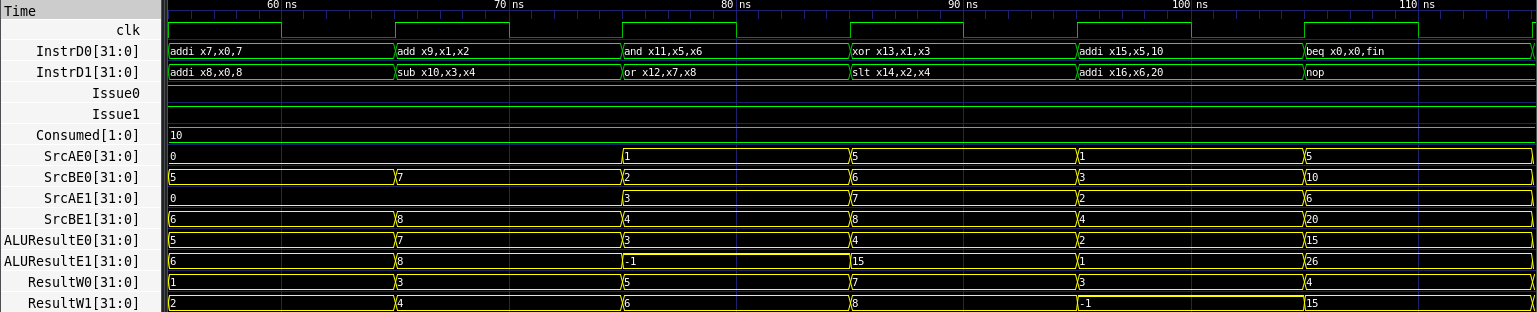
\includegraphics[width=\textwidth]{../img/e2_p6.png}
\caption{Programa 6, de 55 a 115~ns.}
\label{fig:e2p6}
\end{figure}

En la Figura~\ref{fig:e2p6}, \sig{Issue1} permanece en 1 y \sig{Consumed = 10}: sale un par en cada ciclo. A los 70~ns, Decode tiene \sig{add x9, x1, x2} y \sig{sub x10, x3, x4}. A los 80~ns ambas están en EX: la ALU~0 calcula $1+2=3$ y la ALU~1 calcula $3-4=-1$. A los 100~ns \sig{ResultW0} y \sig{ResultW1} entregan esos dos resultados en el mismo ciclo.

\subsection{RAW dentro del par y forwarding entre vías}

\begin{asm}
# RAW dentro del par (no se emparejan) y forwarding entre vias y etapas
        addi x1, x0, 5
        addi x2, x0, 7
        add  x3, x1, x2        # usa x1 y x2 recien calculados: forwarding
        add  x4, x3, x1        # RAW con la instruccion anterior (x3)
        sub  x5, x4, x3
        and  x6, x5, x4
        or   x7, x6, x5
        xor  x8, x7, x6
        slt  x9, x8, x7
        addi x10, x0, 10       # dos escrituras al mismo registro: gana la mas joven
        addi x10, x0, 20
        add  x11, x10, x10     # debe leer 20
        add  x12, x11, x9
        add  x13, x12, x11
        sw   x13, 0(x0)
fin:    beq  x0, x0, fin
\end{asm}

\begin{figure}[htbp]
\centering
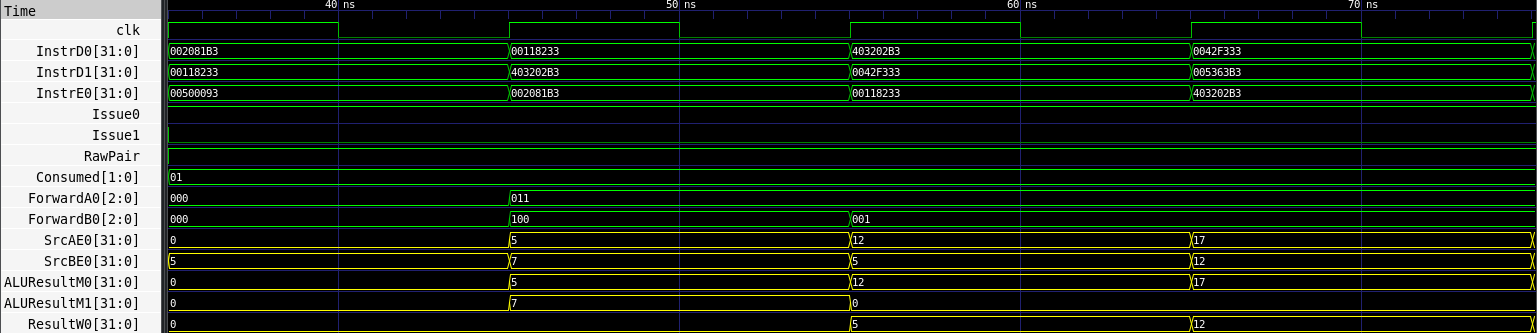
\includegraphics[width=\textwidth]{../img/e2_p7.png}
\caption{Programa 7, de 35 a 75~ns.}
\label{fig:e2p7}
\end{figure}

En la Figura~\ref{fig:e2p7}, a los 40~ns el par es \sig{add x3, x1, x2} y \sig{add x4, x3, x1}. La segunda necesita \sig{x3}, así que \sig{RawPair = 1}, \sig{Issue1 = 0} y \sig{Consumed = 01}. A los 50~ns, la \sig{add x4} ya está en el slot~0 y \sig{add x3} en EX recibe sus operandos de las dos vías de MEM: \sig{ForwardA0 = 011} da el 5 de \sig{ALUResultM0} y \sig{ForwardB0 = 100} da el 7 de \sig{ALUResultM1}. A los 60~ns, \sig{add x4} toma el 12 desde MEM y el 5 desde WB (\sig{ForwardB0 = 001}).

\subsection{Conflicto de memoria y load-use}

\begin{asm}
# load-use y conflictos del puerto de memoria
        addi x1, x0, 11
        addi x2, x0, 22
        sw   x1, 0(x0)
        sw   x2, 4(x0)         # sw + sw: un solo puerto, no se emparejan
        lw   x3, 0(x0)
        add  x4, x1, x2        # lw + ALU independiente: pueden salir juntas
        add  x5, x1, x1
        lw   x6, 4(x0)         # ALU + lw: tambien en el otro orden
        add  x7, x6, x3        # load-use: depende del lw anterior
        sub  x8, x7, x3
        sw   x8, 8(x0)
        lw   x9, 8(x0)
        addi x10, x9, 1        # load-use inmediato
        add  x11, x10, x4
        sw   x11, 12(x0)
fin:    beq  x0, x0, fin
\end{asm}

\begin{figure}[htbp]
\centering
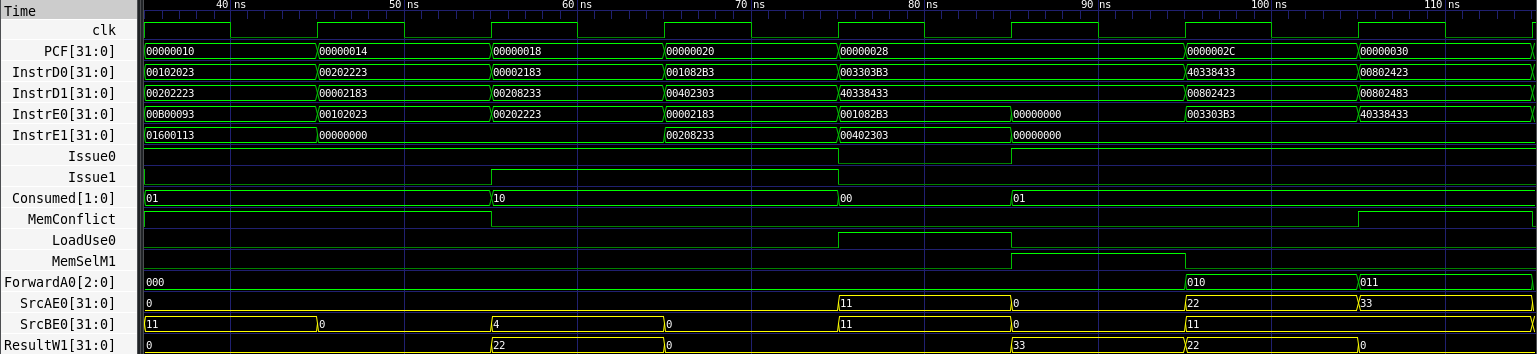
\includegraphics[width=\textwidth]{../img/e2_p8.png}
\caption{Programa 8, de 35 a 115~ns.}
\label{fig:e2p8}
\end{figure}

En la Figura~\ref{fig:e2p8}, a los 40~ns el par son dos \sig{sw}: \sig{MemConflict = 1} y salen en ciclos distintos. A los 60~ns salen juntas \sig{lw x3} y \sig{add x4}, y a los 70~ns, en el orden inverso, \sig{add x5} y \sig{lw x6}, lo que muestra la memoria junto con la ALU en ambas posiciones. Por eso a los 90~ns \sig{MemSelM1 = 1}: el puerto es de la vía~1.

A los 80~ns \sig{add x7, x6, x3} necesita el \sig{lw x6} que está en EX: \sig{LoadUse0 = 1}, \sig{Issue0 = 0} y \sig{Consumed = 00}. A los 90~ns el PC sigue en \sig{0x28}, Decode no cambió y EX tiene burbujas. A los 100~ns, \sig{ForwardA0 = 010} entrega el 22 desde \sig{ResultW1}, que es el dato leído por la vía~1.

\begin{figure}[htbp]
\centering
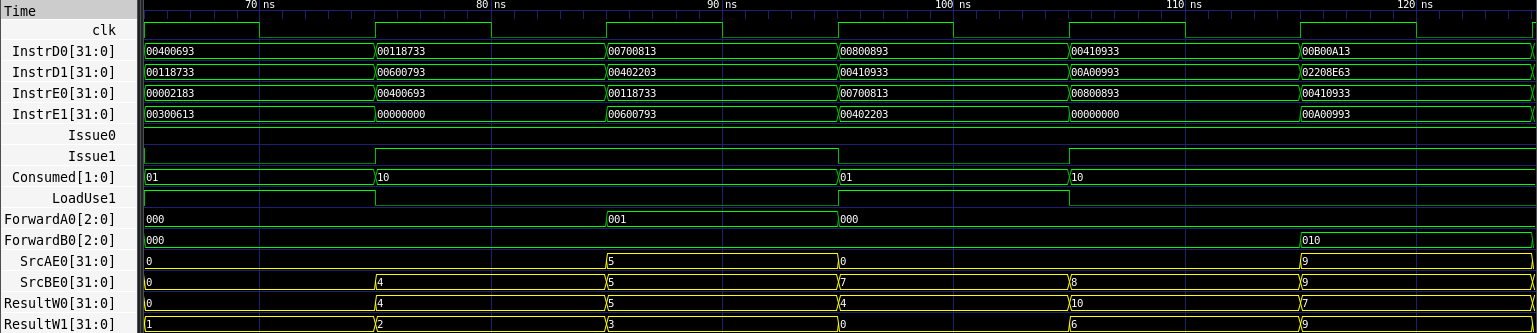
\includegraphics[width=\textwidth]{../img/e2_p13a.png}
\caption{Programa 13, load-use en el slot 1, de 65 a 125~ns.}
\label{fig:e2p13a}
\end{figure}

La Figura~\ref{fig:e2p13a} muestra el load-use en el slot~1. A los 70~ns, \sig{add x14, x3, x1} depende de \sig{lw x3}: \sig{LoadUse1 = 1}, pero el slot~0 es independiente y sale solo (\sig{Consumed = 01}). A los 90~ns, \sig{ForwardA0 = 001} entrega el 5 leído desde \sig{ResultW0}. A los 100~ns ocurre lo mismo con un \sig{lw} en la vía~1, y a los 120~ns el 9 llega por \sig{ResultW1} (\sig{ForwardB0 = 010}).

\subsection{Saltos en ambas posiciones y flushing}

\begin{asm}
# branches en cualquiera de las dos posiciones del par, tomados y no tomados, jal y jalr
        addi x1, x0, 1
        addi x2, x0, 1
        addi x3, x0, 2
        beq  x1, x3, ta        # no tomado
        addi x4, x0, 4
        beq  x1, x2, tb        # tomado: se anula solo lo mas joven
        addi x5, x0, 99
        addi x6, x0, 99
tb:     addi x7, x0, 7
        addi x8, x0, 8
        beq  x7, x8, tc        # no tomado
        addi x9, x0, 9
        nop
        beq  x1, x2, td        # tomado (otra posicion dentro del par)
        addi x11, x0, 99
        addi x12, x0, 99
ta:     addi x13, x0, 99
tc:     addi x14, x0, 99
td:     addi x15, x0, 15
        jal  x16, te           # salto incondicional
        addi x17, x0, 99
        addi x18, x0, 99
te:     addi x19, x0, 104
        jalr x20, 0(x19)       # salto indirecto
        addi x21, x0, 99
        addi x22, x0, 99
tf:     addi x23, x0, 23
        sw   x23, 0(x0)
fin:    beq  x0, x0, fin
\end{asm}

\begin{figure}[htbp]
\centering
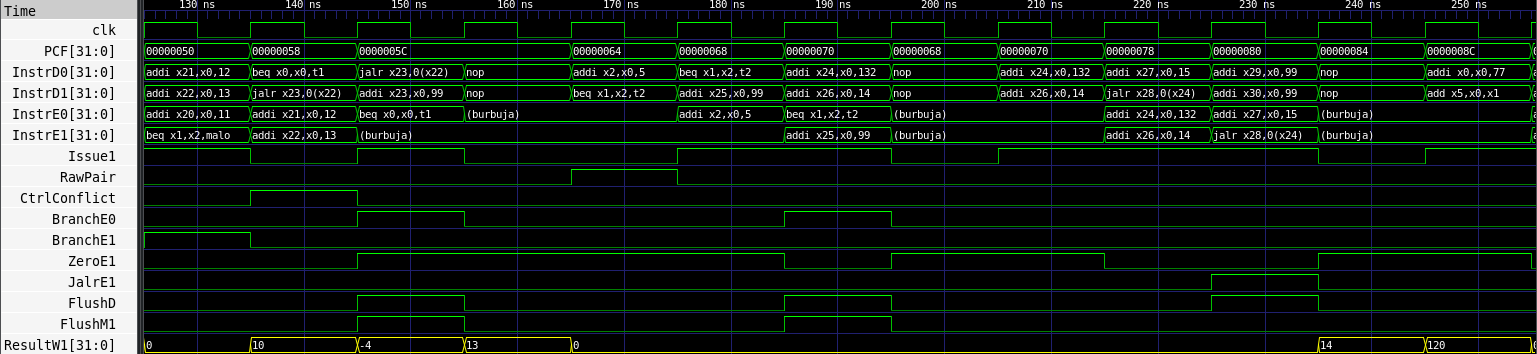
\includegraphics[width=\textwidth]{../img/e2_p13b.png}
\caption{Programa 13, saltos, de 125 a 255~ns.}
\label{fig:e2p13b}
\end{figure}

En la Figura~\ref{fig:e2p13b} aparecen los tres casos:
\begin{itemize}
\item \textbf{No tomado en la vía~1 (130~ns).} \sig{BranchE1 = 1} y \sig{ZeroE1 = 0}, porque $5 \neq 9$. No hay flush y el programa sigue.
\item \textbf{Dos saltos en el par (140~ns).} \sig{beq} y \sig{jalr} levantan \sig{CtrlConflict}. Sale solo el \sig{beq}, que se toma a los 150~ns: \sig{FlushD} y \sig{FlushM1} anulan todo lo posterior. A los 190~ns ocurre otro salto tomado en la vía~0, y \sig{FlushM1} anula la \sig{addi x25} que iba en la vía~1.
\item \textbf{\sig{jalr} en la vía~1 (230~ns).} \sig{JalrE1 = 1} y \sig{FlushD = 1}, pero \sig{FlushM1 = 0}: la \sig{addi x27} de la vía~0 es más antigua y continúa. El PC pasa a \sig{0x84} y a los 250~ns \sig{ResultW1} escribe el enlace 120 (\sig{0x74 + 4}).
\end{itemize}

\subsection{Dos escrituras en el Register File}

\begin{asm}
# dos escrituras al Register File por ciclo y escrituras al mismo registro
        addi x1, x0, 1         # x1 y x2 se escriben en el mismo ciclo (puertos 0 y 2)
        addi x2, x0, 2
        addi x3, x0, 3
        addi x4, x0, 4
        addi x5, x0, 5         # WAW: dos escrituras al mismo registro; gana la mas joven
        addi x5, x0, 6
        addi x6, x0, 7
        addi x6, x0, 8
        add  x7, x5, x6        # 6 + 8
        add  x8, x1, x2
        sw   x7, 0(x0)
        sw   x8, 4(x0)
fin:    beq  x0, x0, fin
\end{asm}

\begin{figure}[htbp]
\centering
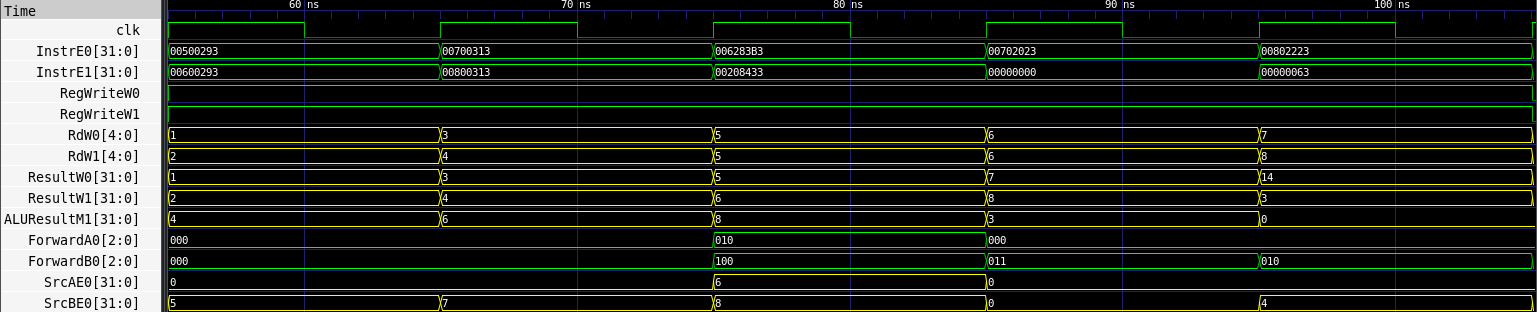
\includegraphics[width=\textwidth]{../img/e2_p10.png}
\caption{Programa 10, de 55 a 105~ns.}
\label{fig:e2p10}
\end{figure}

En la Figura~\ref{fig:e2p10}, \sig{RegWriteW0} y \sig{RegWriteW1} valen 1 a la vez: a los 60~ns se escriben \sig{x1 = 1} y \sig{x2 = 2} en el mismo ciclo. A los 80~ns las dos vías escriben \sig{x5} (5 y 6) y debe ganar la más joven. Justo entonces, \sig{add x7, x5, x6} está en EX y \sig{ForwardA0 = 010} le entrega el 6 de la vía~1. Además, \sig{ForwardB0 = 100} le entrega el 8 de la vía~1 de MEM, y no el 7 de la vía~0, por la misma prioridad.

\subsection{Reagrupamiento y orden de retiro}

\begin{asm}
# emision parcial y reagrupamiento (orden preservado, sin instrucciones perdidas ni repetidas)
        addi x1, x0, 3
        add  x2, x1, x1        # RAW: sale sola, la siguiente se reagrupa
        add  x3, x2, x1
        addi x4, x0, 4         # independiente: puede emparejarse con la anterior
        add  x5, x4, x3
        sw   x5, 0(x0)
        lw   x6, 0(x0)
        sw   x6, 4(x0)         # RAW + memoria
        addi x7, x0, 7
        addi x8, x0, 8
        add  x9, x7, x8
        sub  x10, x9, x7
        sw   x10, 8(x0)
fin:    beq  x0, x0, fin
\end{asm}

\begin{figure}[htbp]
\centering
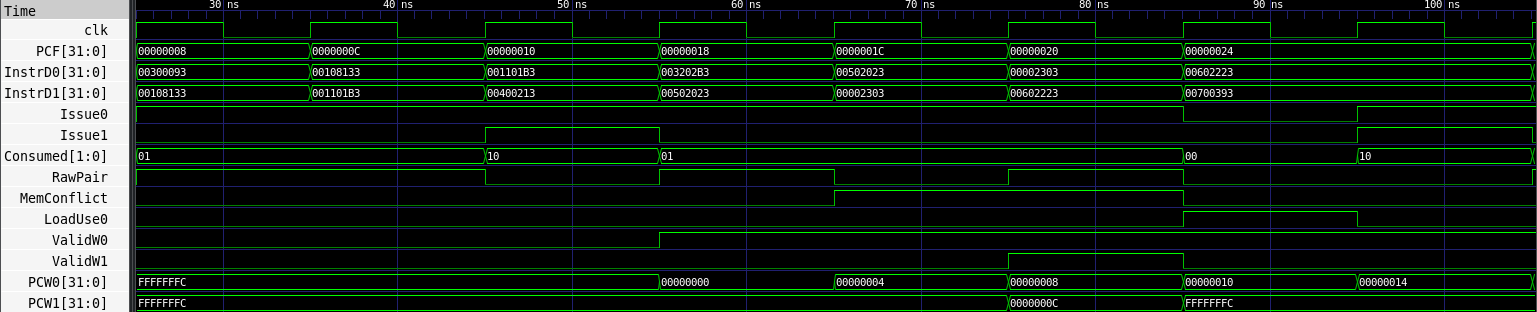
\includegraphics[width=\textwidth]{../img/e2_p11.png}
\caption{Programa 11, de 25 a 105~ns. \sig{PCW = FFFFFFFC} indica que no se retira ninguna instrucción.}
\label{fig:e2p11}
\end{figure}

En la Figura~\ref{fig:e2p11}, de 30 a 40~ns hay \sig{RawPair} y \sig{Consumed = 01}. \sig{InstrD1} pasa a \sig{InstrD0} en el ciclo siguiente y el PC avanza solo 4 (\sig{0x08} a \sig{0x0C}). A los 50~ns se forma un par nuevo con \sig{add x3} y \sig{addi x4}, instrucciones que no venían juntas de Fetch, y salen las dos (\sig{Consumed = 10}, el PC avanza 8). A los 90~ns un load-use congela la ventana (\sig{Consumed = 00}). \sig{PCW0} y \sig{PCW1} muestran el retiro en orden: \sig{0x00}, \sig{0x04}, el par \sig{0x08} y \sig{0x0C}, y luego \sig{0x10} y \sig{0x14}, sin pérdidas ni repeticiones.

% =====================================================================
\section{Comparación con el Single-Issue}
% =====================================================================

La Tabla~\ref{tab:cmp} compara las arquitecturas A (Single-Issue) y B (Dual-Issue) con los mismos programas. Los ciclos se cuentan igual en ambas, desde que baja el reset hasta que se retira la última instrucción del programa, y en los dos casos se comprueba el mismo resultado final. Los testbenches de la arquitectura A están en \sig{Single_Issue} con el sufijo \sig{_single}; ambas versiones se simulan con los pasos del Anexo~A.

\begin{table}[htbp]
\centering
\caption{Ciclos e IPC preliminares. Speedup = ciclos A / ciclos B.}
\label{tab:cmp}
\begin{tabular}{l c c c c c c}
\toprule
\textbf{Programa} & \textbf{Instr.} & \textbf{Ciclos A} & \textbf{Ciclos B} & \textbf{IPC A} & \textbf{IPC B} & \textbf{Speedup} \\
\midrule
1 --- ISA & 29 & 32 & 19 & 0.91 & 1.53 & 1.68 \\
2 --- Forwarding & 7 & 10 & 8 & 0.70 & 0.88 & 1.25 \\
3 --- Stalling & 8 & 12 & 10 & 0.67 & 0.80 & 1.20 \\
4 --- Flushing & 14 & 23 & 18 & 0.61 & 0.78 & 1.28 \\
5 --- Dual Fetch & 11 & 16 & 11 & 0.69 & 1.00 & 1.45 \\
6 --- Dos ALU & 17 & 20 & 12 & 0.85 & 1.42 & 1.67 \\
7 --- RAW & 16 & 19 & 16 & 0.84 & 1.00 & 1.19 \\
8 --- Load y memoria & 16 & 21 & 17 & 0.76 & 0.94 & 1.24 \\
9 --- Branches & 19 & 30 & 23 & 0.63 & 0.83 & 1.30 \\
10 --- Escrituras & 13 & 16 & 10 & 0.81 & 1.30 & 1.60 \\
11 --- Reagrupamiento & 14 & 18 & 15 & 0.78 & 0.93 & 1.20 \\
12 --- Benchmark & 110 & 153 & 133 & 0.72 & 0.83 & 1.15 \\
13 --- Casos vía 1 & 34 & 46 & 31 & 0.74 & 1.10 & 1.48 \\
\bottomrule
\end{tabular}
\end{table}

El mayor speedup aparece donde hay instrucciones independientes: 1.68 en el Programa~1 y 1.67 en el 6. El menor es el del benchmark, 1.15. En sus 110 instrucciones solo se retiraron 20 pares y 70 instrucciones sueltas, con 8 stalls y 17 flushes. Sus lazos tienen dependencias RAW encadenadas y terminan en \sig{beq} y \sig{jal} seguidos, que provocan flushes y no pueden emitirse juntos. Estas son las causas que impiden llegar al IPC ideal de 2.

\subsection{Cómo reproducir las pruebas}

Para simular cada programa se siguen los pasos del Anexo~A, con el código de \sig{Dual_Issue} o \sig{Single_Issue} y los archivos de la Tabla~\ref{tab:repro-e2}. En \sig{Single_Issue}, el testbench lleva el sufijo \sig{_single}.

\begin{table}[htbp]
\centering
\caption{Archivos de cada programa de la Entrega 2.}
\label{tab:repro-e2}
\begin{tabular}{c l l l}
\toprule
\textbf{Programa} & \textbf{Carpeta} & \textbf{Testbench} & \textbf{Programa cargado} \\
\midrule
1 & \sig{Programa1_ISA} & \sig{tb_isa.v} & \sig{isa.mem} \\
2 & \sig{Programa2_Forwarding} & \sig{tb_forwarding.v} & \sig{forwarding.mem} \\
3 & \sig{Programa3_Stalling} & \sig{tb_stalling.v} & \sig{stalling.mem} \\
4 & \sig{Programa4_Flushing} & \sig{tb_flushing.v} & \sig{flushing.mem} \\
5 & \sig{Programa5_DualFetch} & \sig{tb_dualfetch.v} & \sig{dualfetch.mem} \\
6 & \sig{Programa6_DosALU} & \sig{tb_dos_alu.v} & \sig{dos_alu.mem} \\
7 & \sig{Programa7_RAW_Forwarding} & \sig{tb_raw_forwarding.v} & \sig{raw_forwarding.mem} \\
8 & \sig{Programa8_Load_Memoria} & \sig{tb_load_memoria.v} & \sig{load_memoria.mem} \\
9 & \sig{Programa9_Branches} & \sig{tb_branches.v} & \sig{branches.mem} \\
10 & \sig{Programa10_Escrituras} & \sig{tb_escrituras.v} & \sig{escrituras.mem} \\
11 & \sig{Programa11_Reagrupamiento} & \sig{tb_reagrupamiento.v} & \sig{reagrupamiento.mem} \\
12 & \sig{Programa12_Benchmark} & \sig{tb_benchmark.v} & \sig{benchmark.mem} \\
13 & \sig{Programa13_Casos_Via1} & \sig{tb_casos_via1.v} & \sig{casos_via1.mem} \\
\bottomrule
\end{tabular}
\end{table}

\end{document}
